\chapter{Desarrollo del Proyecto}

\section{Arquitectura cliente servidor}

Una arquitectura cliente servidor generalmente considerada como arquitectura
de sistema distribuido. Una vez más, un beneficio importante es la separación
e independencia de funcionalidad. \cite{sommerville2011software}

Esencialmente, el usuario final utiliza un navegador web para solicitar una
página esperando respuesta.

En la figura \ref{Una arquitectura cliente servidor para una filmoteca}, es un
ejemplo de un sistema en base al modelo cliente servidor. 
\cite{sommerville2011software}

\begin{figure}[!htb]
	\centering
	\fbox{
		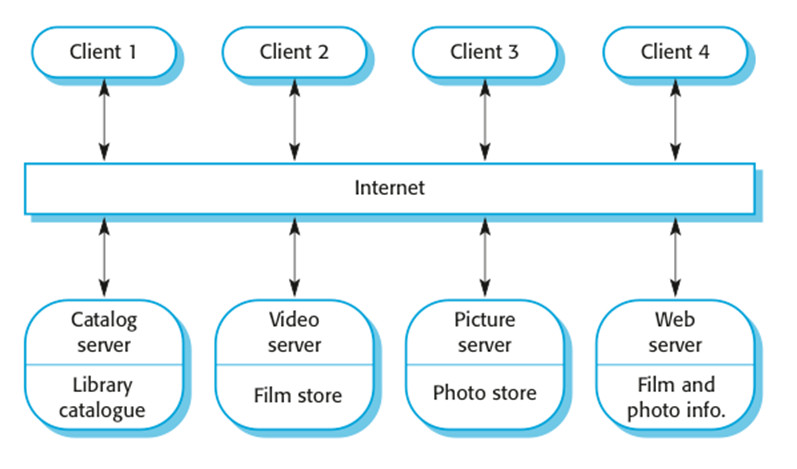
\includegraphics[scale=0.7]{architectureClientServer}
	}
	\caption{Una arquitectura cliente servidor para una filmoteca}
	\source{fuente: \cite{sommerville2011software}}
	\label{Una arquitectura cliente servidor para una filmoteca}
\end{figure}

\subsection{Patrón diseño: modelo vista controlador}

La idea de un patrón es una forma de presentar, compartir y reutilizar el
conocimiento sobre un sistema de software. Se piensa en un patrón
arquitectónico como una estilizada descripción abstracta de buena práctica,
que ha sido probada en diferentes sistemas y entornos. \cite{sommerville2011software}

En la figura \ref{fig:Arquitectura de aplicación web utilizando el patrón MVC},
se muestra una arquitectura de ejecución, cuando este patrón utiliza la
gestión en un sistema basado en la web. \cite{sommerville2011software}

\begin{figure}[ht]
\centering
	\fbox{
		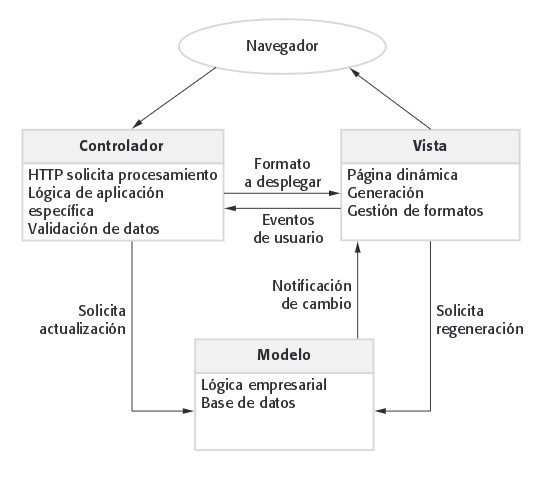
\includegraphics[scale=0.7]{mvcPattern}
	}
	\caption{Arquitectura de aplicación web utilizando el patrón MVC}
	\source{fuente: \cite{sommerville2011software}}
	\label{fig:Arquitectura de aplicación web utilizando el patrón MVC}
\end{figure}


\begin{itemize}

\item \textbf{Diseño del proyecto}

Se considera como patrón base de diseño Modelo Vista Controlador para realizar
la extension de funcionalidad de un Controlador representado como Administrador,
este Administrador realiza una abstracción y re uso de funcionalidad descrito
en la figura \ref{fig:Arquitectura extendida MVCA}.

\begin{figure}[ht]
	\centering
	\fbox{
		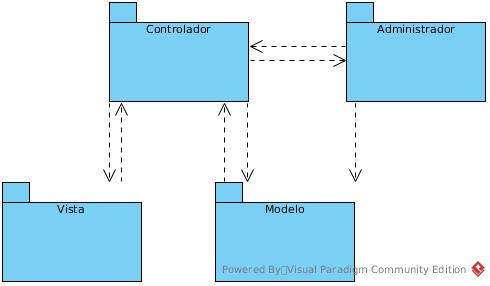
\includegraphics[scale=0.5]{mvcm}
	}
	\caption{Arquitectura extendida MVCA}
	\source{fuente: (Elaboración propia)}
	\label{fig:Arquitectura extendida MVCA}
\end{figure}


\end{itemize}

\section{Designación de rol}

En la plataforma web educativa se implementan cuatro tipos de roles.

\begin{itemize}

\item \textbf{Autorregulado}, rol designado a realizar suscripción o dar de
baja la misma.

\item \textbf{Tutor}, rol designado a un estudiante adscrito de la Carrera de
LAEL, quien tiene la posibilidad de crear podcast de tipo audio/vídeo, agregar
retro alimentación y agregar una transcripción. 

\item \textbf{Coordinador}, rol designado al docente de la Carrera de LAEL, quien
realiza la función de tutor y tiene la posibilidad de crear una categoría.

\item \textbf{Administrador}, rol designado a un adscrito de la Carrera de
Informática, quien tiene la posibilidad de gestionar la seguridad del sistema.

\end{itemize}

\section{Estructura de un podcast} \label{structPodcast}

Un podcast de tipo audio es representado como una estructura que contiene los
siguientes datos.

\begin{itemize}

\item \textbf{título}, nombre representativo, utilizado como identificador.
\item \textbf{imagen de portada}, imagen representativa.
\item \textbf{descripción}, resumen del tema.
\item \textbf{reproductor de audio}, grabación de diálogo.
\item \textbf{fecha de liberación}, fecha de publicación.
\item \textbf{historieta}, imagen de los personajes.
\item \textbf{transcripción}, texto del dialogo.
\item \textbf{actividad}, retro alimentación de actividad.
\item \textbf{resolución}, respuesta de actividad.
\item \textbf{glosario}, descripción de los términos.
\item \textbf{diccionario}, documento de referencia. 

\end{itemize}

Se describe la estructura de un podcast de tipo vídeo; con la diferencia de
tener: transcripción, actividad, resolución de actividad y glosario.

\begin{itemize}

\item \textbf{título}, nombre representativo, utilizado como identificador.
\item \textbf{imagen de portada}, imagen representativa.
\item \textbf{descripción}, resumen del tema.
\item \textbf{reproductor de vídeo}, uso de recursos: imagen, texto y audio.
\item \textbf{fecha liberación}, fecha de publicación.
\item \textbf{infografía}, imágenes descriptivas de tamaño pequeño.
\item \textbf{diccionario}, documento de referencia. 

\end{itemize}

\section{Definición de un componente}

Se considera el siguiente aspecto para describir el proceso de desarrollo.

\begin{itemize}

\item Tarjeta de historia de usuario.
\item Arquitectura de componente.
\item Modelo de componente.
\item Componente.
\item Implementar componente.
\item Problema/Solución de componente.

\end{itemize}

\section{\textquestiondown Cómo implementar un servicio agregado de noticia?} \label{serviceFeed}

La principal tarea de un servicio agregado de noticia es realizar la
notificación vía correo electrónico de nuevo contenido publicado en la web.

En la figura \ref{fig:Arquitectura job queue}, se muestra los componentes de
un servicio agregado de noticia y respectiva comunicación, un proceso en
segundo plano \footnote{segundo plano: Es un programa que se ejecuta sin
intervención del usuario. \cite{background}} se ejecuta respecto la fecha
de liberación descrito en la estructura de un podcast. sección
\ref{structPodcast}

\begin{figure}[!ht]
	\centering
	\fbox{
	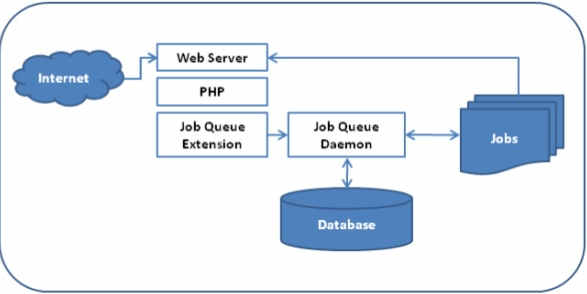
\includegraphics[scale=0.6]{jobQueue}
	}
	\caption{Arquitectura job queue}
	\source{fuente:\cite{ossCamp2014}}
	\label{fig:Arquitectura job queue}
\end{figure}


\subsection{Tarjeta de historia de usuario}

El equipo de informática realizó la elaboración de las historias respecto
a los deseos y sugerencias de un Coordinador de la Carrera de LAEL.

En particular deseo enfatizar los siguientes deseos a realizar:

\begin{itemize}

\item \textbf{Suscripción manual}, tabla: \ref{Tarjeta historia de usuario 03}
\item \textbf{Suscripción de usuario por red social} tabla: 
\ref{Tarjeta historia de usuario 65}.
\item \textbf{Baja de suscripción}, tabla: 
\ref{Tarjeta historia de usuario 60}.
\item \textbf{Liberación de contenido}, tabla: 
\ref{Tarjeta historia de usuario 58}.

\end{itemize}

% add history card 03
\begin{table}[!ht]\centering
\begin{tabular}{|l|l|l|}
\hline
 & \textbf{Tarjeta Historia de Usuario} &  \\ \hline
ID Historia: 03 & \begin{tabular}[c]{@{}l@{}}Nombre: Suscripción a una\\ categoría.\end{tabular} & Fecha: 22/04/2014 \\ \hline
\multicolumn{3}{|l|}{Rol: Aprendiz autorregulado} \\ \hline
\begin{tabular}[c]{@{}l@{}}Modificación de historia\\ número: 05\end{tabular} & \begin{tabular}[c]{@{}l@{}}Iteración asignada: 7,8\end{tabular} & Prioridad en negocio: Medio \\ \hline
Tiempo estimado inicial: 20 & Riesgo en desarrollo: & Tipo de historia: Funcional \\ \hline
\multicolumn{3}{|l|}{\begin{tabular}[c]{@{}l@{}}Descripción:\\ \\ Yo como usuario aprendiz autorregulado deseo suscribirme a un determinado lenguaje \\ (francés básico, ingles básico, quechua básico, quechua psicosocial, fonética quechua), \\tal que me beneficie en recibir notificación de nuevo contenido vía correo. \\ Para esto ya no necesito ingresar mi correo electrónico.\end{tabular}} \\ \hline
\multicolumn{3}{|l|}{\begin{tabular}[c]{@{}l@{}}Pre condición:	\\ \\ Contenido publicado. \\ Servidor SMTP externo configurado.\\ Configuración de credenciales en sistema con servidor SMTP.\end{tabular}} \\ \hline
\multicolumn{3}{|l|}{\begin{tabular}[c]{@{}l@{}}Post condición:\\ \\ Recibir un mensaje en mi bandeja de entrada de mi cuenta de correo.\end{tabular}} \\ \hline
\multicolumn{3}{|l|}{\begin{tabular}[c]{@{}l@{}}Actividades:\\ \\ Desplegar lista de categorías para suscripción.\\ Permitir al usuario seleccionar de la lista de categoría para suscribirse. \\ Guardar suscripción de usuario y registrar fecha.\end{tabular}} \\ \hline
\multicolumn{3}{|l|}{\begin{tabular}[c]{@{}l@{}}Observaciones:\\ \\ La suscripción permite acceder a las noticias de nuevos contenidos de categoría.\end{tabular}} \\ \hline
\begin{tabular}[c]{@{}l@{}}.....................................................\\ Msc. Lic. Vladimir Costas Juaregui\\ PROJECT MANAGER\end{tabular} & \begin{tabular}[c]{@{}l@{}}..........................................\\ Lic. Manuel Camacho Arce\\ PRODUCT OWNER\end{tabular} & \begin{tabular}[c]{@{}l@{}}.........................................\\ Juan Omar Huanca Balboa\\ SCRUM MASTER\end{tabular} \\ \hline
\end{tabular}
\captionof{table}{Tarjeta historia de usuario 03}
\source{fuente: (Elaboración propia)}
\label{Tarjeta historia de usuario 03}
\end{table}

% add history card 65
\begin{table}[!ht]\centering
\begin{tabular}{|l|l|l|}
\hline
 & \textbf{Tarjeta Historia de Usuario} &  \\ \hline
ID Historia: 65 & \begin{tabular}[c]{@{}l@{}}Nombre: Suscripción a una\\ categoría por red social.\end{tabular} & Fecha: 29/08/2016 \\ \hline
\multicolumn{3}{|l|}{Rol: Aprendiz autorregulado} \\ \hline
\begin{tabular}[c]{@{}l@{}}Modificación de historia\\ número: \end{tabular} & \begin{tabular}[c]{@{}l@{}}Iteración asignada: 9, 11\end{tabular} & Prioridad en negocio: Medio \\ \hline
Tiempo estimado inicial: 20 & Riesgo en desarrollo: & Tipo de historia: Funcional \\ \hline
\multicolumn{3}{|l|}{\begin{tabular}[c]{@{}l@{}}Descripción:\\ \\ Yo como usuario aprendiz autorregulado deseo suscribirme a un determinado lenguaje \\ (francés básico, ingles básico, quechua básico, quechua psicosocial, fonética quechua), \\tal que me beneficie en recibir notificación de nuevo contenido vía correo.\\ Para esto necesito pinchar sobre un botón de red social: facebook, google, twitter.\end{tabular}} \\ \hline
\multicolumn{3}{|l|}{\begin{tabular}[c]{@{}l@{}}Pre condición:	\\ \\ Contenido publicado. \\ Usuario autentificado por red social: facebook, google, twitter. \\ Realizar configuración de sistema con en servidor externo: facebook, google, twitter.\end{tabular}} \\ \hline
\multicolumn{3}{|l|}{\begin{tabular}[c]{@{}l@{}}Actividades:\\ \\ Desplegar lista de categorías para suscripción.\\ Permitir al usuario seleccionar de la lista de categoría para suscribirse. \\ Guardar suscripción de usuario y registrar fecha.\end{tabular}} \\ \hline
\multicolumn{3}{|l|}{\begin{tabular}[c]{@{}l@{}}Observaciones:\\ \\ La suscripción permite acceder a las noticias de nuevos contenidos de categoría.\end{tabular}} \\ \hline
\begin{tabular}[c]{@{}l@{}}.....................................................\\ Msc. Lic. Vladimir Costas Juaregui\\ PROJECT MANAGER\end{tabular} & \begin{tabular}[c]{@{}l@{}}..........................................\\ Lic. Manuel Camacho Arce\\ PRODUCT OWNER\end{tabular} & \begin{tabular}[c]{@{}l@{}}.........................................\\ Juan Omar Huanca Balboa\\ SCRUM MASTER\end{tabular} \\ \hline
\end{tabular}
\captionof{table}{Tarjeta historia de usuario 65}
\source{fuente: (Elaboración propia)}
\label{Tarjeta historia de usuario 65}
\end{table}

% this command clear is for !ht table
\clearpage 

% add user history card 60
\begin{table}[!ht]\centering
\begin{tabular}{|l|l|l|}
\hline
 & \textbf{Tarjeta Historia de Usuario} &  \\ \hline
ID Historia: 60 & \begin{tabular}[c]{@{}l@{}}Nombre: Dar de baja \\ suscripción.\end{tabular} & Fecha: 19/05/2015 \\ \hline
\multicolumn{3}{|l|}{Rol: Aprendiz autorregulado} \\ \hline
\begin{tabular}[c]{@{}l@{}}Modificación de historia\\ número: 04\end{tabular} & Iteración asignada: 11 & Prioridad en negocio: Bajo \\ \hline
Tiempo estimado inicial: 15 & Riesgo en desarrollo: & Tipo de historia: Funcional \\ \hline
\multicolumn{3}{|l|}{\begin{tabular}[c]{@{}l@{}}Descripción:\\ \\ Yo como usuario aprendiz autorregulado deseo dar de baja mi suscripción a un determinada \\ categoría tal que me beneficie no recibir más notificación.\\ Para esto necesito pinchar sobre el botón lado la categoría.\end{tabular}} \\ \hline
\multicolumn{3}{|l|}{\begin{tabular}[c]{@{}l@{}}Pre condición:\\ \\ Usuario autentificado. \\ Usuario suscrito\end{tabular}} \\ \hline
\multicolumn{3}{|l|}{\begin{tabular}[c]{@{}l@{}}Post condición:\\ \\ Dejar de recibir notificación a bandeja de correo.\end{tabular}} \\ \hline
\multicolumn{3}{|l|}{\begin{tabular}[c]{@{}l@{}}Actividades:\\ \\ Desplegar la lista de categorías.\\ Verificar registro de categoría.\\ Eliminar registro de suscripción.\\Cambiar estado de suscripción y registrar fecha de baja.\end{tabular}} \\ \hline
\begin{tabular}[c]{@{}l@{}}.....................................................\\ Msc. Lic. Vladimir Costas Juaregui\\ PROJECT MANAGER\end{tabular} & \begin{tabular}[c]{@{}l@{}}..........................................\\ Lic. Manuel Camacho Arce\\ PRODUCT OWNER\end{tabular} & \begin{tabular}[c]{@{}l@{}}.........................................\\ Juan Omar Huanca Balboa\\ SCRUM MASTER\end{tabular} \\ \hline
\end{tabular}
\captionof{table}{Tarjeta historia de usuario 60}
\source{fuente: (Elaboración propia)}
\label{Tarjeta historia de usuario 60}
\end{table}

% add user history card 58
\begin{table}[H]\centering
\begin{tabular}{|l|l|l|}
\hline
 & \textbf{Tarjeta Historia de Usuario} &  \\ \hline
ID Historia: 58 & \begin{tabular}[c]{@{}l@{}}Nombre: Liberación \\ de contenido\end{tabular} & Fecha: 03/05/2015 \\ \hline
\multicolumn{3}{|l|}{Rol: Tutor} \\ \hline
\begin{tabular}[c]{@{}l@{}}Modificación de historia\\ número:\end{tabular} & Iteración asignada: 10 & Prioridad en negocio: Medio \\ \hline
Tiempo estimado inicial: 35 & Riesgo en desarrollo: & Tipo de historia: Funcional \\ \hline
\multicolumn{3}{|l|}{\begin{tabular}[c]{@{}l@{}}Descripción:\\ \\ Yo como usuario tutor deseo realizar la automática publicación de mi contenido tal que se \\ publiquen de acuerdo a fecha indicada en el registro.\end{tabular}} \\ \hline
\multicolumn{3}{|l|}{\begin{tabular}[c]{@{}l@{}}Pre condición:	\\ \\ Usuario autentificado. \\Contenido registrado. \\ Fecha actual de sistema debe ser mayor a fecha de liberación de contenido.\end{tabular}} \\ \hline
\multicolumn{3}{|l|}{\begin{tabular}[c]{@{}l@{}}Actividades: \\ \\ Generar un script para obtener los contenidos inhabilitados \\ Enviar un mensaje de notificación a los usuarios suscritos a categoría respectiva.\\ Cambiar estado de contenido en habilitado.\end{tabular}} \\ \hline
\multicolumn{3}{|l|}{\begin{tabular}[c]{@{}l@{}}Observaciones:\\ \\ La liberación de contenido debe estar condicionado a fecha de liberación.\end{tabular}} \\ \hline
\begin{tabular}[c]{@{}l@{}}.....................................................\\ Msc. Lic. Vladimir Costas Juaregui\\ PROJECT MANAGER\end{tabular} & \begin{tabular}[c]{@{}l@{}}..........................................\\ Lic. Manuel Camacho Arce\\ PRODUCT OWNER\end{tabular} & \begin{tabular}[c]{@{}l@{}}.........................................\\ Juan Omar Huanca Balboa\\ SCRUM MASTER\end{tabular} \\ \hline
\end{tabular}
\captionof{table}{Tarjeta historia de usuario 58}
\source{fuente: (Elaboración propia)}
\label{Tarjeta historia de usuario 58}
\end{table}

\subsection{Arquitectura de componente}

\begin{itemize}

\item \textbf{Suscripción manual}
en la figura \ref{fig:Diagrama de caso de uso registrar suscripción de usuario},
las acciones del rol autorregulado realiza el requerimiento descrito en tabla
\ref{Tarjeta historia de usuario 03}.

\begin{figure}[!ht]
	\centering
	\fbox{
		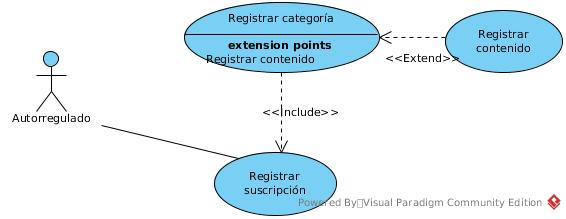
\includegraphics[scale=0.6]{useCaseRegisterSubscription}
	}
	\captionof{figure}{Diagrama de caso de uso registrar suscripción manual}
	\source{fuente: (Elaboración propia)}
	\label{fig:Diagrama de caso de uso registrar suscripción de usuario}
\end{figure}

\item \textbf{Suscripción y baja de suscripción}
en la figura \ref{fig:Diagrama de caso de uso para personalizar suscripción, dar baja},
las acciones del rol autorregulado realiza el requerimiento descrito en tablas
\ref{Tarjeta historia de usuario 65} y \ref{Tarjeta historia de usuario 60}.

\begin{figure}[!ht]
	\centering
	\fbox{
		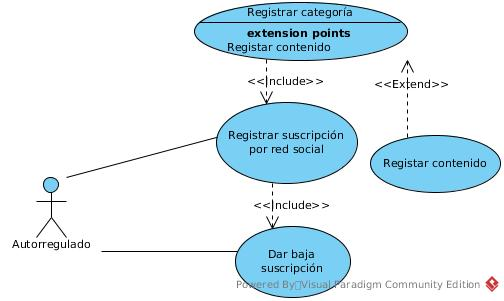
\includegraphics[scale=0.6]{useCaseSubscriptionUnsubscription}
	}
	\captionof{figure}{Diagrama de caso de uso para personalizar suscripción, dar baja}
	\source{fuente: (Elaboración propia)}
	\label{fig:Diagrama de caso de uso para personalizar suscripción, dar baja}
\end{figure}

\item \textbf{Liberación de contenido} en la figura 
\ref{fig:Diagrama de caso de uso para liberación de contenido}, la acción del
rol tutor realiza la definición de fecha de liberación y el proceso cron
ejecuta el script descrito en tabla \ref{Tarjeta historia de usuario 58}.

\begin{figure}[!ht]
	\centering
	\fbox{
		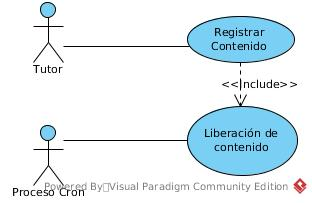
\includegraphics[scale=0.7]{useCaseRelease}
	}
	\captionof{figure}{Diagrama de caso de uso para liberación de contenido}
	\source{fuente: (Elaboración propia)}
	\label{fig:Diagrama de caso de uso para liberación de contenido}
\end{figure}

\item \textbf{Suscripción manual}
en la figura \ref{fig:Diagrama de clase para suscripción de usuario}, el diagrama
representa la composición de datos y comunicación de las clases.

\begin{figure}[H]
	\centering
	\fbox{
		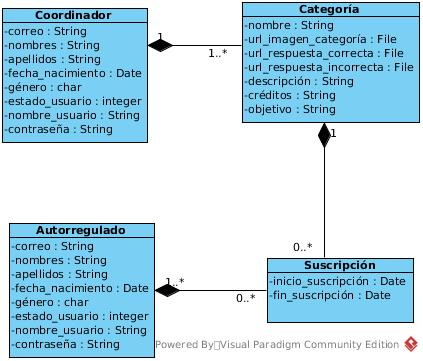
\includegraphics[scale=0.6]{classRegisterSubscription}
	}
	\captionof{figure}{Diagrama de clase para suscripción manual}
	\source{fuente: (Elaboración propia)}
	\label{fig:Diagrama de clase para suscripción de usuario}
\end{figure}

\item \textbf{Suscripción, baja de suscripción y liberación de contenido}
en la figura \ref{fig:Diagrama de clase para suscriptor}, el diagrama
representa la composición de datos y comunicación de las clases.

\begin{figure}[!ht]
	\centering
	\fbox{
		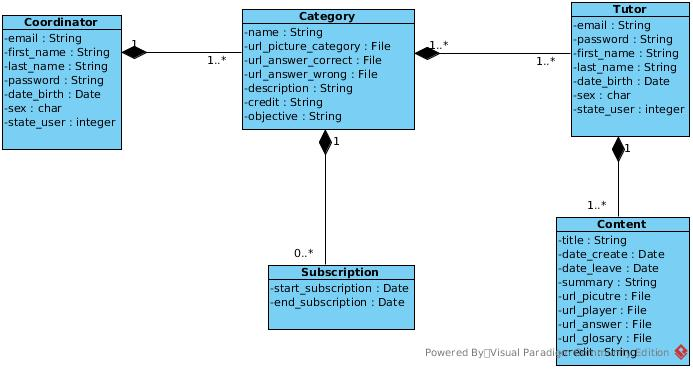
\includegraphics[scale=0.6]{classSubscription}
	}
	\captionof{figure}{Diagrama de clase para suscripción}
	\source{fuente: (Elaboración propia)}
	\label{fig:Diagrama de clase para suscriptor}
\end{figure}

\item \textbf{Suscripción manual}
en la figura \ref{fig:Diagrama de secuencia para suscripción}, el diagrama
de secuencia representa la comunicación del rol autorregulado con las
diferentes clases.

\begin{figure}[H]
	\centering
	\fbox{
		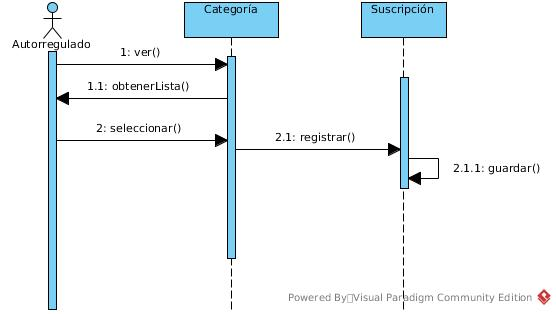
\includegraphics[scale=0.7]{sequenceRegisterSubscription}
	}
	\captionof{figure}{Diagrama de secuencia para suscripción manual}
	\source{fuente: (Elaboración propia)}
	\label{fig:Diagrama de secuencia para suscripción}
\end{figure}

\item \textbf{Suscripción y baja de suscripción}
en la figura \ref{fig:Diagrama de secuencia para suscripción}, el diagrama
de secuencia representa la comunicación del rol autorregulado con las
diferentes clases.

\begin{figure}[!ht]
	\centering
	\fbox{
		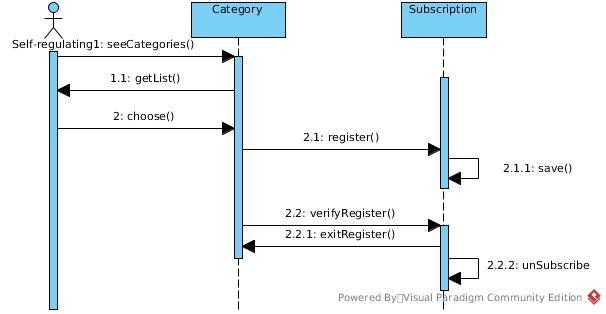
\includegraphics[scale=0.7]{sequenceSubscription}
	}
	\captionof{figure}{Diagrama de secuencia para suscripción}
	\source{fuente: (Elaboración propia)}
	\label{fig:Diagrama de secuencia para suscripción}
\end{figure}


\item \textbf{Liberación de contenido}
en la figura \ref{fig:Diagrama de secuencia para liberación de contenido},
el diagrama de secuencia representa la comunicación del rol tutor con las
diferentes clases, el proceso cron verifica el registro de contenido para
luego ejecutar un script.

\begin{figure}[!ht]
	\centering
	\fbox{
		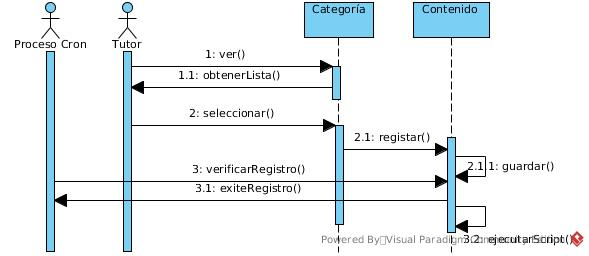
\includegraphics[scale=0.7]{sequenceRelease}
	}
	\captionof{figure}{Diagrama de secuencia para liberación de contenido}
	\source{fuente: (Elaboración propia)}
	\label{fig:Diagrama de secuencia para liberación de contenido}
\end{figure}

\end{itemize}

\subsection{Modelo de componente}

\begin{itemize}

\item \textbf{Suscripción manual} 
en la figura \ref{fig:Modelo de datos para suscripción de usuario}, el modelo de datos
representa la persistencia de suscripción de categoría y suscripción por
red social.

\begin{figure}[!ht]
	\centering
	\fbox{
		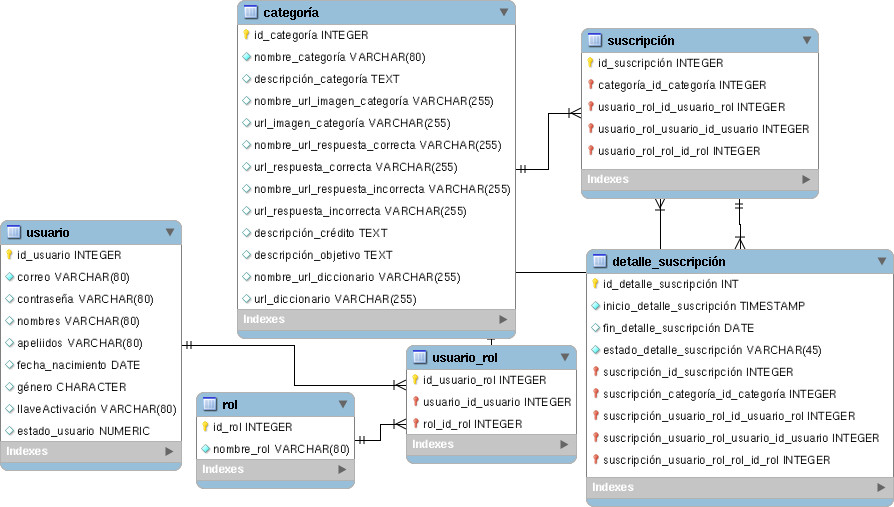
\includegraphics[scale=0.5]{modelRegisterSubscription}
	}
	\captionof{figure}{Modelo de datos para suscripción de usuario}
	\source{fuente: (Elaboración propia)}
	\label{fig:Modelo de datos para suscripción de usuario}
\end{figure}

La suscripción conformado por categoría genera una bitácora \footnote{bitácora:
Mecanismo persistencia de actividades en el tiempo. (Elaboración propia)}
y detalle\textunderscore suscripción.

\item \textbf{Suscripción y baja de suscripción}
en la figura \ref{fig:Modelo de datos para suscriptor}, el modelo de datos
representa la persistencia de suscripción de categoría y suscripción por
red social.

\begin{figure}[!ht]
	\centering
	\fbox{
		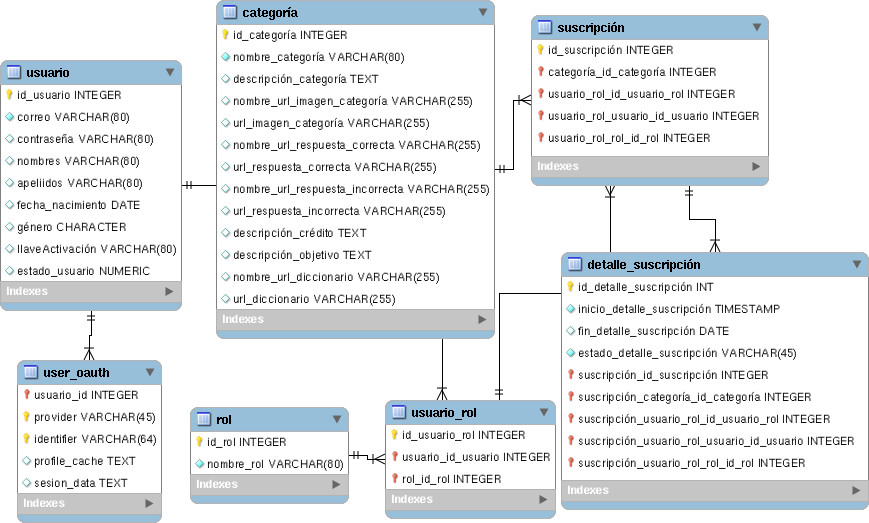
\includegraphics[scale=0.5]{modelSubscription}
	}
	\captionof{figure}{Modelo de datos para suscriptor}
	\source{fuente: (Elaboración propia)}
	\label{fig:Modelo de datos para suscriptor}
\end{figure}

\item \textbf{Liberación de contenido}
en la figura \ref{fig:Modelo de datos para liberación de contenido},
el modelo de datos representa la persistencia de registro de contenido
y fecha de liberación.

\begin{figure}[!ht]
	\centering
	\fbox{
		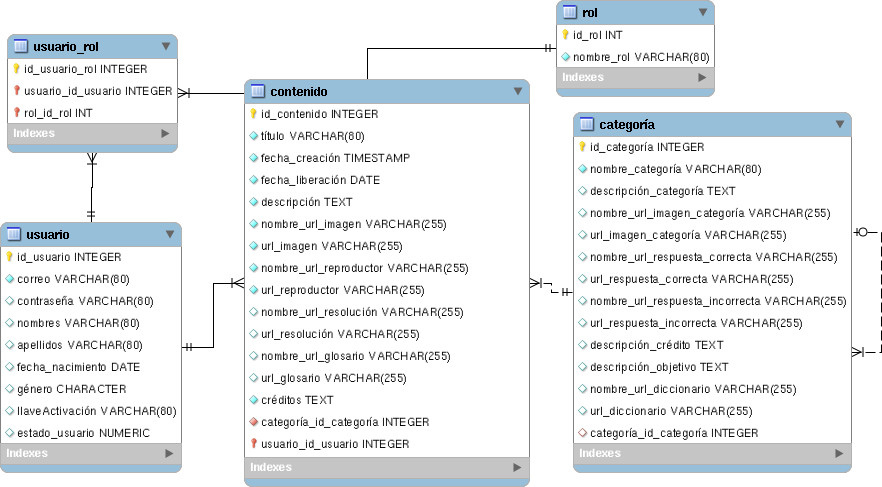
\includegraphics[scale=0.5]{modelRelease}
	}
	\captionof{figure}{Modelo de datos para liberación de contenido}
	\source{fuente: (Elaboración propia)}
	\label{fig:Modelo de datos para liberación de contenido}
\end{figure}


\end{itemize}

\subsection{Componente}

\begin{itemize}

\item \textbf{Suscripción}
se propone la primera opción para realizar una suscripción.

\begin{itemize}

\item \textbf{Manual}, permite realizar la suscripción con una dirección de
correo sujeto a verificación de sistema.

\end{itemize}

\textbf{Manual} en la figura \ref{fig:Ventana emergente de suscripción}, se
representa un formulario de registro de dirección de correo electrónico para
realizar una suscripción. 

\begin{figure}[!ht]
	\centering
	\fbox{
		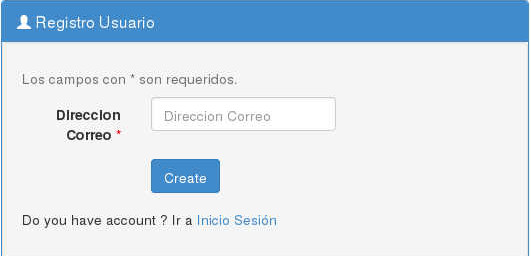
\includegraphics[scale=0.7]{modalSubscribe}
	}
	\captionof{figure}{Ventana emergente de suscripción}
	\source{fuente: (Elaboración propia)}
	\label{fig:Ventana emergente de suscripción}
\end{figure}

\item \textbf{Suscripción de usuario}
se propone la segunda opción para realizar una suscripción.

\begin{itemize}

\item \textbf{Token de red social}, permite realizar la suscripción con un
servicio externo provisto por redes sociales de google, facebook y twitter.

\end{itemize}

\textbf{Token \footnote{Token: Se clasifica como una de las cinco clases de
fichas que describen sus funciones (constantes, identificadores, operadores,
palabras reservadas y separadores) de acuerdo con las reglas del lenguaje de
programación. \cite{token}} de red social} en la figura \ref{fig:Formulario
de inicio de sesión}, el formulario de inicio de sesión tiene la funcionalidad
de ingresar a su entorno de trabajo.

\begin{figure}[H]
	\centering
	\fbox{
		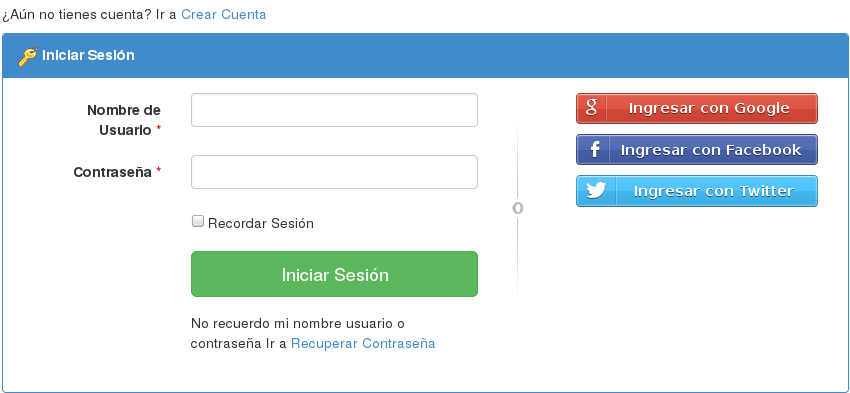
\includegraphics[scale=0.6]{login}
	}
	\captionof{figure}{Formulario de inicio de sesión}
	\source{fuente: (Elaboración propia)}
	\label{fig:Formulario de inicio de sesión}
\end{figure}

\begin{enumerate}

\item \textbf{Facebook}, en la figura \ref{fig:Aplicación de sesión para facebook},
el flujo en un servidor de facebook para realizar el acceso de una cuenta válida.

\begin{figure}[!ht]
	\centering
	\fbox{
		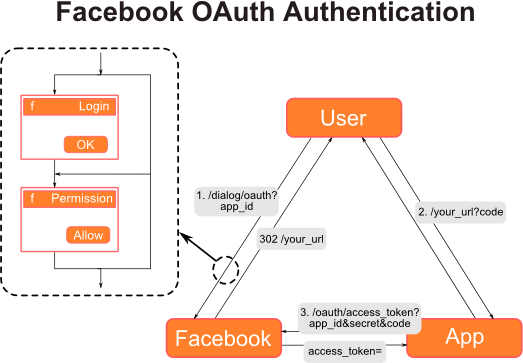
\includegraphics[scale=0.5]{oauthFacebook}
	}
	\captionof{figure}{Aplicación de sesión para facebook}
	\source{fuente: \cite{oauthFacebook}}
	\label{fig:Aplicación de sesión para facebook}
\end{figure}

\item \textbf{Google}, en la figura \ref{fig:Aplicación de sesión para google}, el
diagrama secuencia facilita el acceso para una cuenta válida de un usuario.

\begin{figure}[!ht]
	\centering
	\fbox{
		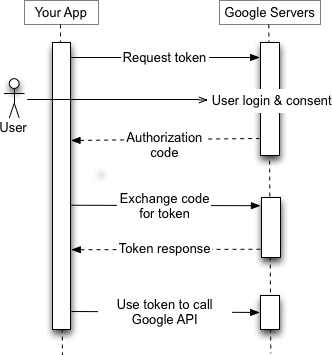
\includegraphics[scale=0.7]{oauth20Google}
	}
	\captionof{figure}{Aplicación de sesión para google}
	\source{fuente: \cite{oauthGoogle}}
	\label{fig:Aplicación de sesión para google}	
\end{figure}

\item \textbf{Twitter}, en la figura \ref{fig:Aplicación de sesión para twitter},
el flujo dentro un servidor de twitter permite realizar el inicio de sesión de
una cuenta de usuario.

\begin{figure}[!ht]
	\centering
	\fbox{
		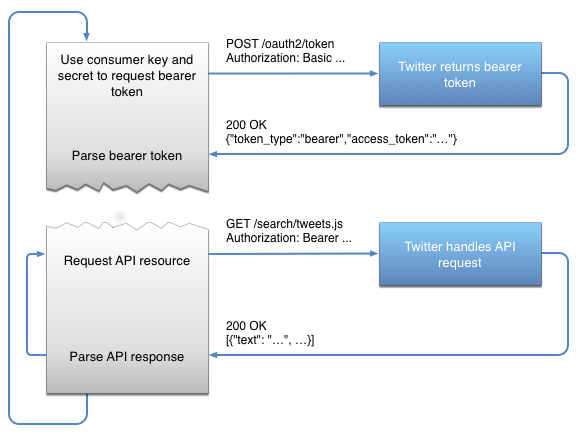
\includegraphics[scale=0.5]{oauth10Twitter}
	}
	\captionof{figure}{Aplicación de sesión para twitter}
	\source{fuente: \cite{oauthTwitter}}
	\label{fig:Aplicación de sesión para twitter}
\end{figure}

\end{enumerate}

\item \textbf{Baja suscripción} en la figura 
\ref{fig:Suscripción programa aprendizaje francés básico}, un usuario de
sistema suscrito a una categoría (francés básico) desea dar de baja su
respectiva suscripción. Para el mismo solo se tiene que pinchar sobre el botón
\textquotedouble{Suscrito}. 

\begin{figure}[!ht]
	\centering
	\fbox{
		
\includegraphics[scale=0.6]{basicFranceSubscribed}
	}
	\captionof{figure}{Suscripción programa aprendizaje francés básico}
	\source{fuente: (Elaboración propia)}
	\label{fig:Suscripción programa aprendizaje francés básico}
\end{figure}


\item \textbf{Liberación de contenido} en la figura
\ref{fig:Formulario registro de contenido}, el formulario de registro de
contenido permite definir la fecha de liberación del propio contenido.

\begin{figure}[H]
	\centering
	\fbox{
		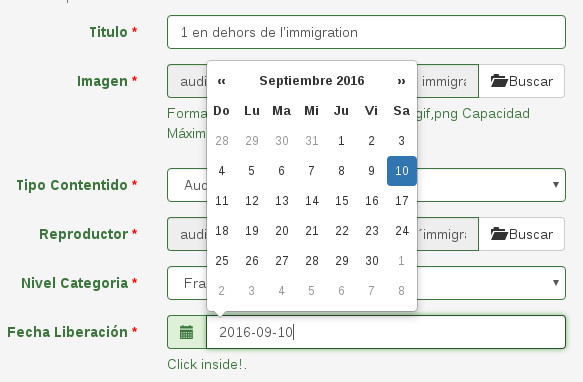
\includegraphics[scale=0.7]{formContent}
	}
	\captionof{figure}{Formulario registro de contenido}
	\source{fuente: (Elaboración propia)}
	\label{fig:Formulario registro de contenido}
\end{figure}

\end{itemize}
	
\subsection{Implementar componente}

\begin{itemize}

\item \textbf{Suscripción - implementar en el servidor} el
siguiente segmento de código permite personalizar la suscripción por
categoría, el suscriptor obtiene las categorías habilitadas. 

\begin{lstlisting}[language=PHP, caption={Personalización de suscriptor.}]
public function actionCustomRss($idCategory) {
    ob_end_clean();
    header('Content-type: text/xml; charset=utf-8');
    $this->layout = false;    // turn off layout
    $criteria = new CDbCriteria;     // add custom criteria
    $criteria->addCondition('t.category_id_category=:Column1');
    $criteria->addCondition('t.category_id_category in (select i.category_id_category
    from interest as i) and t.content_status=' . Yii::app()->params[
    'stateContentAvailable']);
    $criteria->select = 't.title,t.summary,t.date_leave';
    $criteria->params = array(':Column1' => $idCategory);
    $data = Content::model()->findAll($criteria);
    $this->renderPartial('_viewItemChannel', array(
        'data' => $data,
    ));     // redirect view
}
\end{lstlisting}

En la linea dos tiene la funcionalidad limpiar buffer de salida y
des habilitar su uso.

En la linea tres agrega la cabecera de un documento XML y codificación con
el formato UTF-8 \footnote{UTF-8: El estándar Unicode cubre todos
los caracteres, signos de puntuación y símbolos en el mundo. Unicode 
procesamiento, almacenamiento y transporte de texto, independiente de la 
plataforma y lenguaje \cite{utf8}}.

\item \textbf{Baja de suscripción - implementar en el servidor} el siguiente
segmento de código verifica el registro de una suscripción, si la verificación
es verdadera realiza la baja, caso contrario registra nueva suscripción.
\begin{lstlisting}[language=PHP, caption={Verificación registro suscripción.}]
public function actionVerifySubscribeCategory() {
$user_id_user = Yii::app()->user->id; // get user id
...
foreach ($model_user_rols as $model_user_rol) { // iterate each row UserRol
    ...
    $model_subscription = Subscription::model()->findByAttributes(array(
    'category_id_category' => $category_id_category, 'id_user_rol' => 
    $id_user_rol, 'rol_id_rol' => $rol_id_rol, 'user_id_user' => $user_id_user));
    $manager_detail_subscription = new DetailSubscriptionManager();
    if ($model_subscription == null) { // verify array is null
        $model_subscription = new Subscription('create'); // new model Interest
        ...
        if ($model_subscription->validate()) { // verify valitation
            $this->saveModel($model_subscription); // save tuple
            ...
        }
    } else {
        $model_detail_subscription = DetailSubscription::model()->findByAttributes
        (array('subscription_id_subscription' => $model_subscription->
        id_subscription, 'subscription_category_id_category' => 
        $category_id_category, 'subscription_user_id_user' => $user_id_user,
        'status_detail_subscription' => Yii::app()->params[
        'stateDetailSubscribeAvailable']));
        if ($model_detail_subscription == null) { // verify change
            ...
        }
    }
}    
}
\end{lstlisting}

\item \textbf{Liberación de contenido - implementar en el servidor} el
proceso cron utiliza una tabla para la definición para una tarea, la
instrucción realiza ejecución de un script para liberación de diferentes
podcasts.

Ejecutar el comando sobre una terminal. A continuación se debe iniciar sesión
como usuario \textquotedouble{root}.

\begin{lstlisting}[language=bash, caption={Acceso archivo crontab.}]
# contrab -e
\end{lstlisting}

\textbf{sobre una sola línea} el comando a ejecutar tiene la siguiente sintaxis
de minuto (0-59) hora (0-23) día del mes (1-31) mes del año (1-12) día de la
semana (0-7) comando/script/tarea a ejecutar.

\begin{lstlisting}[language=bash, caption={Comando para ejecución de tarea.}]
0 0 * * * php /var/www/html/plataformaeducativalael/protected/utils/job.php job
\end{lstlisting}

A continuación la función principal del script job.php, obtiene podcast
a ser liberado. Enviar una notificación por correo a los usuarios suscritos.

\begin{lstlisting}[language=PHP, caption={Método principal de clase JobCommand.}]
public function run($args) {
    $jobs = $this->getJobs();
    foreach ($jobs as $job) {
        Yii::log("Running - Job [". $job->title ."] scheduled for ".
        $job->date_create, 'info', 'jobprocessor');
        $job->content_status = Yii::app()->params['stateContentAvailable'];
        $job->save(); // save data
        $this->sendMailSubscribed($job->category_id_category, $job->user_id_user,
        $job->title, $job->summary);
    }
}
\end{lstlisting}

\end{itemize}

\subsection{Problema/Solución de componente}

\begin{itemize}

\item \textbf{Suscripción manual} la dificultad surgió para implementar.

\begin{itemize}

\item Generación única de modal \footnote{modal: Una ventana modal es,
por tanto, normalmente una ventana secundaria. El usuario tiene interarticular
con el antes de que el control se pueda devolver a la solicitud principal.
\cite{modal}} para cada categoría.

\end{itemize}

La ventana modal utiliza el identificador de la categoría hija, para una lista
de categorías hijas pinchar sobre el botón de la ultima categoría realiza la
replica de identificador sobre los demás elementos.

\begin{enumerate}

\item \textbf{Generar único identificador por modal - implementar en el cliente}
como mecanismo de solución se generara un identificador conformado por
categoría padre y categoría hija.

\begin{lstlisting}[language=HTML, caption={Generador ventana modal.}]
<?php $this->beginWidget(
        'booster.widgets.TbModal', array(
    'id' => 'myModal' . $category_id,
));?>
<div class="modal-body">
    <div class="panel-body">
        <?php $this->renderPartial('//site/createRegisterSuscribe', 
        array('model_user' => $model_user)); ?>
    </div>
</div>
<?php $this->endWidget(); ?>
\end{lstlisting}

El problema de notificación vía correo electrónico se genera por las etiquetas
propias de HTML \footnote{HTML: Es el conjunto de símbolos de marcado o
códigos insertados en un archivo destinado a la visualización de una página
web mundial. \cite{html}}.

\end{enumerate}

\item \textbf{Baja de suscripción} la dificultad se obtuvo al momento de implementar.
\begin{itemize}
\item Estado usuario botón suscripción.
\end{itemize}
\begin{enumerate}
\item \textbf{Estado usuario botón suscripción - implementar en el cliente}
en el segmento de código se utiliza una variable local para almacenar el valor
de una categoría suscrita y realizar el cambio según la verificación de registro
de usuario.
\begin{lstlisting}[language=PHP, caption={Cambio de estado botón de suscripción.}]
$category_id_result = 0;
foreach ($model_detail_subscriptions as $model_detail_subscription){
    if ($model_detail_subscription->subscription_category_id_category ==
            $category_id){
        $category_id_result = $category_id;
    }
}
$this->widget(
'booster.widgets.TbButton', array(
'label' => ($category_id_result == $category_id) ?'<i class="fa fa-rss"></i> '.
    Yii::t('app', 'Subscribed') :'<i class="fa fa-rss"></i> '. Yii::t('app', 
    'Subscribe'),
'context' => 'warning',
'encodeLabel'=>false,        
'htmlOptions' => array(
    'id' => 'button' . $category_id,
    'data-dismiss' => 'modal',
    'class'=>'btn-subscribe',
    'ajax' => array(
        'type' => 'POST',
        'url' => $this->createUrl('subscription/verifySubscribeCategory'),
        'success' => 'js:function(data){ $("#button' . $category_id . '").html("'
        . Yii::t("app", "Subscribed") . '");}',
        'data' => array(
            'idCategory' => 'js:$("#user-formRegisterSuscribe' . $category_id 
                . ' #User_category_id").val()',
        ),
    ),
),
'encodeLabel' => false)
);
\end{lstlisting}

\end{enumerate}

\item \textbf{Liberación de contenido}

\begin{itemize}

\item Envió de mensaje de notificación.
\item Obtener contenido sujeto a condición de liberación. 

\end{itemize}

\begin{enumerate}

\item \textbf{Envió de mensaje - implementar en el servidor}

El segmento de código implementa el envió de correo, tiene la característica
de mostrar un mensaje sin página maestra.

\begin{lstlisting}[language=PHP, caption={Envió de mensaje sin  contenedor de página.}]
private function sendMailSubscribed($idCategory, $idUser, $title, $summary) {
$userRols = Category::model()->getRecentUserSubscribe($idCategory);
foreach ($userRols->categoryUserRol as $userRol) {
    if ($idUser != $userRol->user_id_user) {
        $subject = Yii::app()->params['setSubjectContentRelease'];
        $body = Yii::app()->params['setBodyContentRelease'] . $title . $summary
        . Yii::app()->params['setBodyBelowContentRelease'] 
        . Yii::app()->params['adminEmail']
        . Yii::app()->params['setBodyBottomContentRelease'];
        $to = $userRol->userIdUser->email;
        $mail = new YiiMailer(); // send mail
        $mail->setBody($body); //use cron view from views/mail
        $mail->setData(array('message' => $subject, 'name' => get_class($this), 
        'description' => 'Cron job', 'mailer' => $mail));
        $mail->render(); //render HTML mail, layout is set from config file
        $mail->From = Yii::app()->params['adminEmail'];
        $mail->FromName = Yii::app()->params['fromNameConsole'];
        $mail->Subject = $subject;
        $mail->AddAddress($to);
        if ($mail->send()) { // send
            Yii::log(Yii::app()->params['succeedSendContentRelease']); 
        } else {
            Yii::log(Yii::app()->params['wrongSendContenRelease']);
        }
    }
}
}
\end{lstlisting}

\item \textbf{Obtención de contenido - implementar en el servidor}
en el segmento de código se realiza el uso de la función \textquotedouble{scopes}
para obtener contenido habilidad y la fecha de sistema es mayor la fecha
de liberación.

\begin{lstlisting}[language=PHP, caption={Obtención de contenido para liberar podcast.}]
public function scopes() {
return array(
    'active' => array(
        'condition' => 'content_status='.Yii::app()->params[
            'stateContentUnavailable'],
    ),
    'current' => array(
        'condition' => 'date_leave < now()',
    ),
);
}
\end{lstlisting}

\end{enumerate}

\end{itemize}

\section{\textquestiondown Cómo implementar un glosario y subtitulado?}

Relacionar un reproductor de podcast de tipo audio con su transcripción
genera un efecto de subtitulado. 

Definir un glosario de términos con significado.
 
\subsection{Tarjeta de historia de usuario}

El equipo de informática realizó la elaboración de las historias respecto
a los deseos y sugerencias de un Coordinador de la Carrera de LAEL.

En particular deseo enfatizar los siguientes deseos a realizar:

\begin{itemize}

\item \textbf{Gestionar glosario de podcast}, tabla
\ref{Tarjeta historia de usuario 64}.
\item \textbf{Gestionar subtitulado de podcast audio}, tabla 
\ref{Tarjeta historia de usuario 66}.

\end{itemize}

% add user history card 64
\begin{table}[!ht]\centering
\begin{tabular}{|l|l|l|}
\hline
 & \textbf{Tarjeta Historia de Usuario} &  \\ \hline
ID Historia: 64 & \begin{tabular}[c]{@{}l@{}}Nombre: Registrar\\ glosario audio podcast\end{tabular} & Fecha: 19/05/2015 \\ \hline
\multicolumn{3}{|l|}{Rol: Tutor} \\ \hline
\begin{tabular}[c]{@{}l@{}}Modificación de historia\\ número: 04\end{tabular} & Iteración asignada: 13,14 & Prioridad en negocio: Medio \\ \hline
Tiempo estimado inicial: 30 & Riesgo en desarrollo: & Tipo de historia: Funcional \\ \hline
\multicolumn{3}{|l|}{\begin{tabular}[c]{@{}l@{}}Descripción:\\ \\ Yo como usuario tutor deseo gestionar un glosario tal que me beneficie en la definición de \\términos.\\ Para esto necesito: frase, lenguaje destino, significado.\end{tabular}} \\ \hline
\multicolumn{3}{|l|}{\begin{tabular}[c]{@{}l@{}}Pre condición:\\ \\ Usuario autentificado. \\ Contenido registrado.\end{tabular}} \\ \hline
\multicolumn{3}{|l|}{\begin{tabular}[c]{@{}l@{}}Como probarlo: \\ \\ pinchar sobre la segunda opción definición glosario dentro de la opción.\end{tabular}} \\ \hline
\multicolumn{3}{|l|}{\begin{tabular}[c]{@{}l@{}}Actividades:\\ \\Pinchar sobre la opción Administrar mis contenidos. \\ Pinchar sobre la opción traducción.\\ Seleccionar la opción de glosario. \\Llenar los valores de formulario. \\ Guardar registro glosario.\end{tabular}} \\ \hline
\begin{tabular}[c]{@{}l@{}}.....................................................\\ Msc. Lic. Vladimir Costas Juaregui\\ PROJECT MANAGER\end{tabular} & \begin{tabular}[c]{@{}l@{}}..........................................\\ Lic. Manuel Camacho Arce\\ PRODUCT OWNER\end{tabular} & \begin{tabular}[c]{@{}l@{}}.........................................\\ Juan Omar Huanca Balboa\\ SCRUM MASTER\end{tabular} \\ \hline
\end{tabular}
\captionof{table}{Tarjeta historia de usuario 64}
\source{fuente: (Elaboración propia)}
\label{Tarjeta historia de usuario 64}
\end{table}

% use command for table !ht
\clearpage

% add user history card 66
\begin{table}[H]\centering
\begin{tabular}{|l|l|l|}
\hline
 & \textbf{Tarjeta Historia de Usuario} &  \\ \hline
ID Historia: 66 & \begin{tabular}[c]{@{}l@{}}Nombre: Registrar\\ subtitulado podcast\end{tabular} & Fecha: 09/05/2015 \\ \hline
\multicolumn{3}{|l|}{Rol: Tutor} \\ \hline
\begin{tabular}[c]{@{}l@{}}Modificación de historia\\ número:\end{tabular} & Iteración asignada: 15,16 & Prioridad en negocio: Medio \\ \hline
Tiempo estimado inicial: 35 & Riesgo en desarrollo: & Tipo de historia: Funcional \\ \hline
\multicolumn{3}{|l|}{\begin{tabular}[c]{@{}l@{}}Descripción:\\ \\ Yo como usuario tutor deseo tener un subtitulado tal que me beneficie poder relacionar\\ reproductor con transcripción de un podcast.\\ \\ Para esto necesito:frase, lenguaje destino, significado, tiempo inicio y tiempo fin.\end{tabular}} \\ \hline
\multicolumn{3}{|l|}{\begin{tabular}[c]{@{}l@{}}Pre condición:	\\ \\ Usuario Autentificado.\end{tabular}} \\ \hline
\multicolumn{3}{|l|}{\begin{tabular}[c]{@{}l@{}}Como probarlo:\\ \\ Pinchar sobre el reproductor, pinchar dos veces sobre el botón mostrar/ocultar traducción para \\ poder ver la transcripción y una traducción a un lenguaje destino.\end{tabular}} \\ \hline
\multicolumn{3}{|l|}{\begin{tabular}[c]{@{}l@{}}Actividades:\\ \\Pinchar sobre la opción Administrar mis contenidos. \\ Pinchar sobre la opción traducción.\\ Seleccionar la opción de frase. \\Llenar los valores de formulario. \\ Pinchar sobre el reproductor para definir tiempos: inicio, fin. \\ Guardar registro glosario.\end{tabular}} \\ \hline\begin{tabular}[c]{@{}l@{}}.....................................................\\ Msc. Lic. Vladimir Costas Juaregui\\ PROJECT MANAGER\end{tabular} & \begin{tabular}[c]{@{}l@{}}..........................................\\ Lic. Manuel Camacho Arce\\ PRODUCT OWNER\end{tabular} & \begin{tabular}[c]{@{}l@{}}.........................................\\ Juan Omar Huanca Balboa\\ SCRUM MASTER\end{tabular} \\ \hline
\end{tabular}
\captionof{table}{Tarjeta historia de usuario 66}
\source{fuente: (Elaboración propia)}
\label{Tarjeta historia de usuario 66}
\end{table}

\subsection{Arquitectura de componente}

En la figura \ref{fig:Diagrama de caso de uso para glosario y subtitulado},
el diagrama de caso de uso representa la accion de un rol autorregulado
para definición de requerimiento descrito en tabla
\ref{Tarjeta historia de usuario 64} y tabla
\ref{Tarjeta historia de usuario 66}

\begin{figure}[H]
	\centering
	\fbox{
		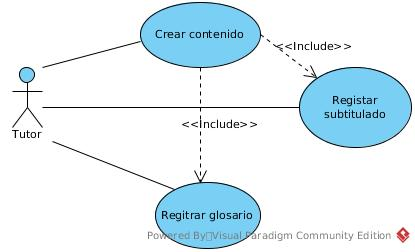
\includegraphics[scale=0.7]{useCaseTranslation}
	}
	\captionof{figure}{Diagrama de caso de uso para glosario y subtitulado}
	\source{fuente: (Elaboración propia)}
	\label{fig:Diagrama de caso de uso para glosario y subtitulado}
\end{figure}

En la figura \ref{fig:Diagrama de clases para glosario y subtitulado},
el diagrama de clases representa la abstracción de datos y comunicación
de clases.

%\begin{figure}[H]
\begin{figure}[!ht]
	\centering
	\fbox{
		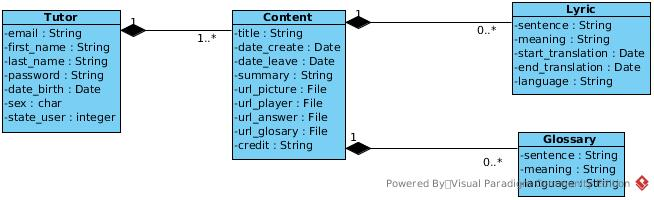
\includegraphics[scale=0.7]{classTranslation}
	}
	\captionof{figure}{Diagrama de clases para glosario y subtitulado}
	\source{fuente: (Elaboración propia)}
	\label{fig:Diagrama de clases para glosario y subtitulado}
\end{figure}

En la figura \ref{fig:Diagrama de secuencia para glosario y subtitulado},
el diagrama de secuencia representa la comunicación de un rol autorregulado
y las clases de glosario y subtitulado.

\begin{figure}[H]
	\centering
	\fbox{
		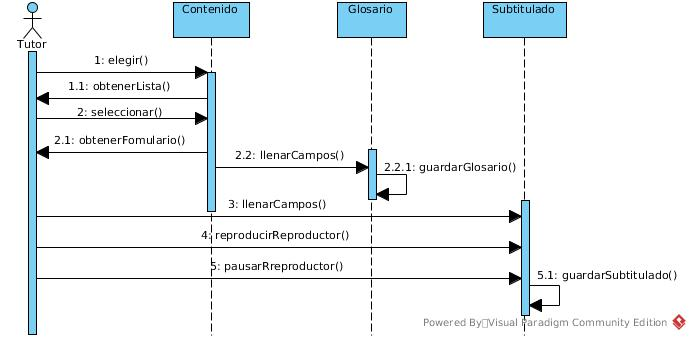
\includegraphics[scale=0.6]{sequenceTranslation}
	}
	\captionof{figure}{Diagrama de secuencia para glosario y subtitulado}
	\source{fuente: (Elaboración propia)}
	\label{fig:Diagrama de secuencia para glosario y subtitulado}
\end{figure}

\subsection{Modelo de componente}

En la figura \ref{fig:Modelo de datos para glosario y subtitulado}, el modelo
de datos representa la persistencia de glosario y subtitulado.

\begin{figure}[!ht]
	\centering
	\fbox{
		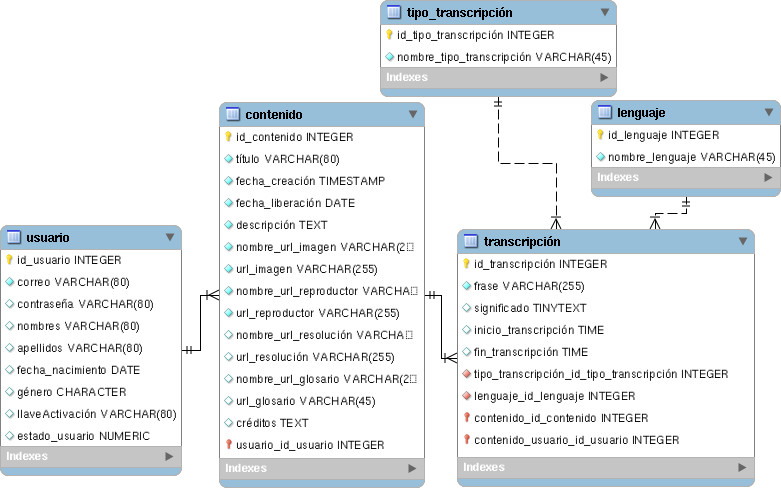
\includegraphics[scale=0.6]{modelTranslation}
	}
	\captionof{figure}{Modelo de datos para glosario y subtitulado}
	\source{fuente: (Elaboración propia)}
	\label{fig:Modelo de datos para glosario y subtitulado}
\end{figure}

\subsection{Componente}

\begin{itemize}

\item \textbf{Glosario de sentencia}, permite crear una frase con respectivo
significado.
\item \textbf{Subtitulado de transcripción}, permite relacionar reproductor
de tipo audio con transcripción.

\end{itemize}

\textbf{Glosario} en la figura \ref{fig:Formulario de registro para glosario}, el
formulario brinda la funcionalidad de crear glosario; considerando lo
siguientes campos de tipo, frase, lenguaje destino y significado.

\begin{figure}[!ht]
	\centering
	\fbox{
		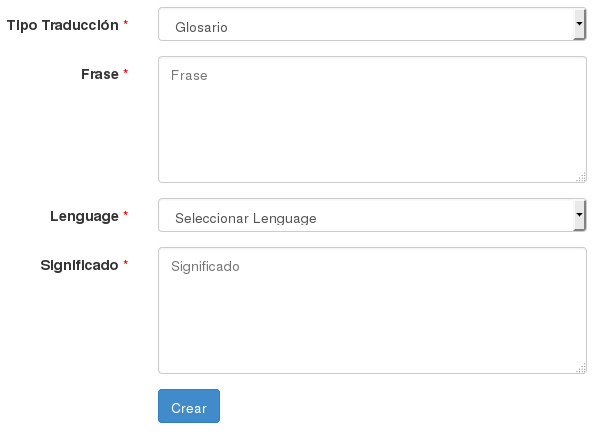
\includegraphics[scale=0.6]{formGlossary}
	}
	\captionof{figure}{Formulario de registro para glosario}
	\source{fuente: (Elaboración propia)}
	\label{fig:Formulario de registro para glosario}
\end{figure}

\textbf{Subtitulado} en la figura \ref{fig:Formulario de registro para subtitulado},
el formulario permite la creación de un subtitulado conformado de frase, lenguaje
destino, significado, reproductor, tiempo inicio y tiempo fin.

\begin{figure}[H]
	\centering
	\fbox{
		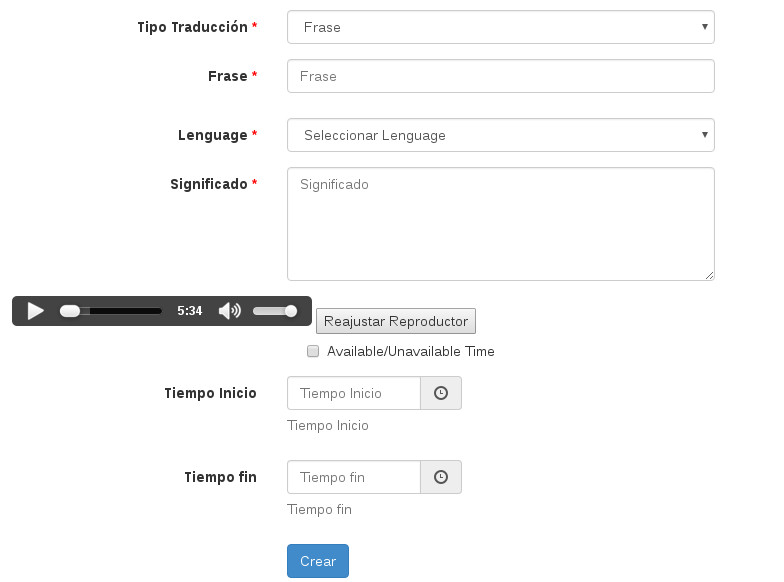
\includegraphics[scale=0.6]{formLyric}
	}
	\captionof{figure}{Formulario de registro para subtitulado}
	\source{fuente: (Elaboración propia)}
	\label{fig:Formulario de registro para subtitulado}
\end{figure}

En la figura \ref{fig:Diagrama de estado para subtitulado}, el diagrama de
esto representa los diferentes estados que tiene un reproductor para la
definición de los tiempos de un subtitulado. 

\begin{figure}[!ht]
	\centering
	\fbox{
		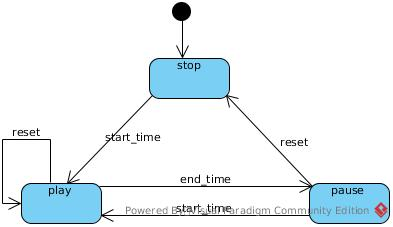
\includegraphics[scale=0.7]{stateLyric}
	}
	\captionof{figure}{Diagrama de estado para subtitulado}
	\source{fuente: (Elaboración propia)}
	\label{fig:Diagrama de estado para subtitulado}
\end{figure}

\subsection{Implementar componente}

\begin{itemize}

\item \textbf{Subtitulado - implementar en el cliente} el segmento de código
obtiene dos listas de transcripción origen y traducción destino.

\begin{lstlisting}[caption={Llenado de elemento en subtitulado.}, label={lst:fillSubtitle}]
var myPlayer = document.getElementById("audio-player"); // get object audio player
var flag = false; // flag for run one time
myPlayer.addEventListener("play", function () { // add event play listener
if (!flag) { // verify no change flag
    $.ajax({ // get property through ajax
        type: "POST",
        url: "<?php echo CController::createUrl('Translation/getItemSentences');
        ?>",
        data: {
            idTypeTranslation: "<?php echo Yii::app()->params[
                'idTypeTranslationSentence']; ?>",
            idContent: "<?php echo Yii::app()->getRequest()->getParam(
                    'id_content'); ?>",
            idUser: "<?php echo Yii::app()->getRequest()->getParam(
                    'user_id_user'); ?>",
            idLanguage: "<?php echo $model_translation->language_id_language; ?>"
    },
    dataType: "html",
    success: function (data) {
    var div = document.getElementById("idSentence");
    div.innerHTML = data;
    }
    });
    .....
    flag = true; // change flag
    play(myPlayer); // call function for show subtitle
}
}, false);
\end{lstlisting}

\item \textbf{Subtitulado - implementar en el cliente} el segmento de código
realiza la acción necesaria para mostrar/ocultar el subtitulado de podcast,
por lo cual el botón realizar el evento de control.

\begin{lstlisting}[caption={Control de mostrar/ocultar subtitulado.}]
function play(myPlayer) {
    var controlDuplicate = [];
    myPlayer.ontimeupdate = function () {
    var currentTimePhrase = myPlayer.currentTime; // get currentTime player
    var currentIDStart = ""; // identifier for start_translation, end_translation
    var currentIDEnd = "";
    var timeConvert = ""; // time converter min:seg
    var hr = Math.floor(currentTimePhrase / 3600); //convert from seg to min
    var min = Math.floor((currentTimePhrase - (hr * 3600)) / 60);
    var sec = Math.floor(currentTimePhrase - (hr * 3600) - (min * 60));
    if (min < 10) { // if min is less 10 add 0
        min = "0" + min;
    }
    if (sec < 10) { // if sec is less 10 add 0
        sec = "0" + sec;
    }
    timeConvert = min + ':' + sec + ':00';
    if (controlDuplicate.length == 0) {
        controlDuplicate.push(timeConvert);
    $('#idSentence li').filter(':not([start_time_translation]),
        [start_time_translation="' + timeConvert + '"]').addClass(
        'sentence_show');
    ...
    } else if (controlDuplicate[controlDuplicate.length - 1] != timeConvert) {
        controlDuplicate.push(timeConvert);
    $('#idSentence li').filter(':not([start_time_translation]),
        [start_time_translation="'+ timeConvert + '"]').addClass(
        'sentence_show');
    $('#idSentence li').filter(':not([start_time_translation]),
        [end_time_translation="' + timeConvert + '"]').removeClass(
        'sentence_show');
    ...
    }
    };
}
\end{lstlisting}

\end{itemize}

\subsection{Problema/Solución de componente}

\begin{itemize}

\item \textbf{Glosario de término}

\begin{itemize}

\item Uso de registro de un solo formulario para la definición de glosario y
subtitulado.

\end{itemize}

\begin{enumerate}

\item \textbf{Validación de campos en formulario} en el segmento de código
la validación de un escenario para glosario se definido en el modelo de clase.

\begin{lstlisting}[language=PHP, caption={Validación de campos para escenario glosario.}]
public function actionCreate($id_content, $id_user) {
...
if (isset($_POST['Translation'])) {
    $model->attributes = $_POST['Translation'];
    $model->content_id_content = $id_content; // fill property
    $model->content_user_id_user = $id_user;
    if ($_POST['Translation']['type_translation_id_type_translation'] == 
            Yii::app()->params['idTypeTranslationSentence']) {
        $model->setScenario('sentence'); //change scenary
        $model->start_translation = $_POST['Translation']['start_translation'];
        $model->end_translation = $_POST['Translation']['end_translation'];
    } elseif ($_POST['Translation']['type_translation_id_type_translation'] == 
            Yii::app()->params['idTypeTranslationDictionary']) {
        $model->setScenario('dictionary'); //change scenary
    }
    if ($model->validate()) {
        $this->saveModel($model);
        ...
    }
}
...
}
}
\end{lstlisting}

\end{enumerate}

\item \textbf{Subtitulado de reproductor}

\begin{itemize}

\item Definición de formato de hora de minutos para tiempo inicio y
minuto tiempo final.
\item Frase de transcripción de tiempo inicio y tiempo final.

\end{itemize}

\begin{enumerate}

\item \textbf{Formato de hora} el reproductor define el valor a través de
la acción reproducir/detener, de manera que el tiempo debe considerar el
siguiente formato de mm:ss

Por tanto la unidad de tiempo obtenida de un reproductor es insuficiente para
esto agregar un cero por delante.

\begin{lstlisting}[caption={Generador de formato para minuto y segundo.}]
var myPlayer = document.getElementById("playerMyTranslation");
myPlayer.addEventListener("play", function () {
    var status_start_translation = document.getElementById(
        'start_translation').disabled;
    if (!status_start_translation) {
        var second_start_translation = Math.floor(myPlayer.
            currentTime % 60);
        if (second_start_translation < 10) {
            second_start_translation = "0" + 
            second_start_translation;
        }
        var minute_start_translation = Math.floor((myPlayer.currentTime / 60)
                % 60);
        if (minute_start_translation < 10) {
            minute_start_translation = "0" + 
            minute_start_translation;
        }
        document.getElementById('start_translation').value = 
                minute_start_translation +':' + second_start_translation;
        }
}, false);
...
\end{lstlisting}

\item \textbf{Revertir valor de inicio} el usuario con rol tutor puede
realizar una equivocación al momento definir el evento del reproductor,
para esto se recomienda revertir con el siguiente segmento de código.

\begin{lstlisting}[caption={Revertir valor de tiempo y reproductor.}]
function resetPlayer() {
    var status_start_translation = document.getElementById(
        'start_translation').disabled;
    var status_end_translation = document.getElementById(
        'end_translation').disabled;
    var myPlayer = document.getElementById("playerMyTranslation");
    if (!status_start_translation && !status_end_translation) {
        if (myPlayer.play) {
        myPlayer.currentTime = 0;
        document.getElementById('start_translation').value = 0; // set start
        document.getElementById('end_translation').value = 0; // set end
        }
    }
}
\end{lstlisting}

\end{enumerate}

\end{itemize}

\section{\textquestiondown Cómo representar glosario y subtitulado?}

Se agrega contenido semántico a: glosario y subtitulado. 

\subsection{Componente}

\begin{itemize}

\item \textbf{Representación de glosario uso de h-entry}
el esquema de representación de un micro-formato de tipo h-entry para la
representación de un glosario de podcast. \cite{hEntry}

\begin{itemize}

\item \textbf{p-name} nombre entrada/título.
\item \textbf{p-summary} breve resumen entrada.
\item \textbf{e-content} contenido completo entrada.
\item \textbf{dt-published} cuando se publicó la entrada.
\item \textbf{dt-updated} cuando se actualiza la entrada.
\item \textbf{p-author} que escribió la entrada, opcional mente incorporados
h-card.
\item \textbf{p-category} categoría entrada tags.
\item \textbf{u-url} URL del enlace permanente entrada.
\item \textbf{u-uid} identificador único universal, la entrada URL canónica
normalmente.
\item \textbf{p-location} la ubicación de la entrada fue publicada a partir,
opcional mente embed h-card, or h-geo.
\item \textbf{u-syndication} URL de copias sindicatos de este post, La propiedad
equivalente de rel-syndication.
\item \textbf{u-in-reply-to} la URL cual h-entry se considera respuesta a, 
opcional mente una h-cite.

\end{itemize}

En la figura \ref{fig:Presentación glosario}, el glosario podcast tiene como
elementos de frase y significado. 

\begin{figure}[!ht]
	\centering
	\fbox{
		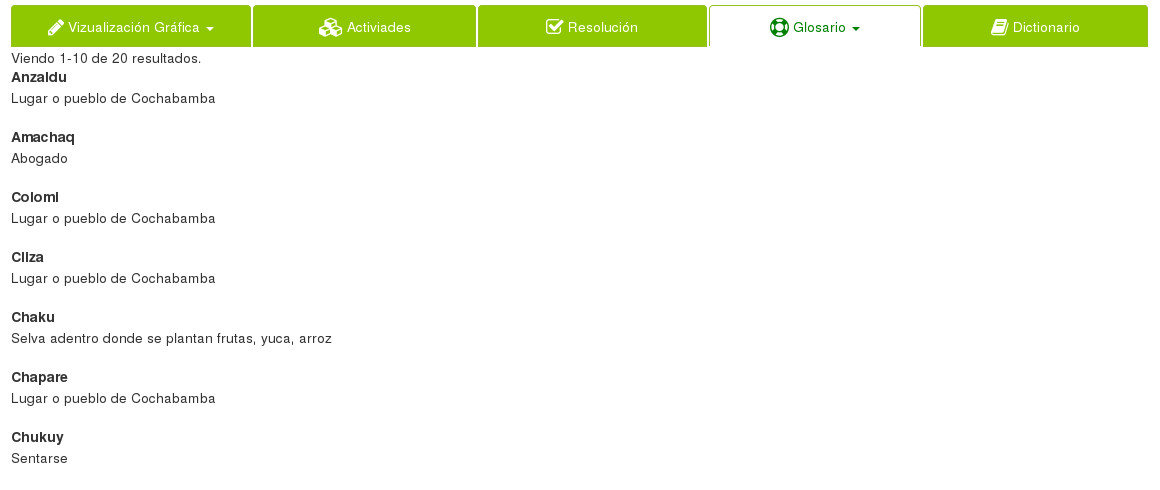
\includegraphics[scale=0.5]{glossary}
	}
	\captionof{figure}{Presentación glosario}
	\source{fuente: (Elaboración propia)}
	\label{fig:Presentación glosario}
\end{figure}

\item \textbf{Representación de subtitulado} microformato tiene una
cantidad definida de tipos, se debe utilizar microformato 2 considerado
como extension de funcionalidad. 

\textbf{microformato 2}

\begin{itemize}

\item 'h-*' de nombres de clase raíz.
\item 'p-*' para las características simples (texto).
\item 'u-*' para las características URL.
\item 'dt-*' para la características de fecha/hora.
\item 'e-*' para las propiedades de marcado incrustado. \cite{microformats2}
 
\end{itemize}

Se propone la siguiente estructura para agregar contenido semántico para un
subtitulado.

\begin{enumerate}

\item \textbf{h-x-lyrics} raíz de esquema.

	\begin{enumerate}
	
		\item \textbf{p-lyric h-x-lyric} contenedora de elementos.
		
			\begin{enumerate}

				\item \textbf{p-start-time} representa tiempo inicio.
				\item \textbf{p-content} representa contenido.
				\item \textbf{p-end-time} representa tiempo fin.			

				\end{enumerate}					

	\end{enumerate}

\end{enumerate}

En la figura \ref{fig:Representación de subtitulado}, el reproductor de audio
sincroniza con subtitulado.

\begin{figure}[!ht]
	\centering
	\fbox{
		
\includegraphics[scale=0.6]{lyric}
	}
	\captionof{figure}{Representación de subtitulado}
	\source{fuente: (Elaboración propia)}
	\label{fig:Representación de subtitulado}
\end{figure}

\end{itemize}

\subsection{Implementar componente}

\begin{itemize}

\item \textbf{Glosario - implementar en el cliente} el segmento de código
agrega contenido semántico para glosario tiene un microformato de tipo
h-entry.

\begin{lstlisting}[language = PHP, caption={Representación de glosario.}]
<dl class="h-entry">
    <dt class="p-name">
        <?php echo $data->sentence; ?> 
    </dt> 
    <dd class="p-content">
        <?php echo $data->meaning; ?> 
    </dd>
</dl>
\end{lstlisting}

\item \textbf{Subtitulado - implementar en el cliente} el segmento de código
describe la agregación de la estructura propuesta para subtitulado.

\begin{lstlisting}[language = PHP, caption={Estructura de sentencia.}]
<ul class="h-sentence-lyrics ul_hide">
    <?php foreach ($model_translations as $translation): ?>  
    <li class="p-lyric h-sentence-lyric"> 
        <time class="p-start-time"> <?php echo $translation->start_translation;
        ?> </time>    
        <span class="p-content" > <?php echo $translation->sentence; ?></span>
        <time class="p-end-time"> <?php echo $translation->end_translation;?> 
           </time>
    </li>
    <?php endforeach; ?>
</ul>
...
\end{lstlisting}

\end{itemize}

\subsection{Problema/Solución de componente}

\begin{itemize}

\item \textbf{Representación de glosario}

\begin{itemize}

\item Uso de HTML5 \footnote{HTML5: Es una versión del lenguaje de marcado
de hipertexto, el lenguaje de programación estándar para describir el
contenido y la apariencia de las páginas web. \cite{html5}}  para agregar 
contenido semántico.

\begin{enumerate}

\item \textbf{Uso de estándar HTML5} el uso de documento HTML5 permite el
uso estándar para microformato.

\end{enumerate}

\end{itemize}

\item \textbf{Representación de subtitulado}

\begin{itemize}

\item Agregación de microformato en el lado del servidor.

\end{itemize}

\begin{enumerate}
 
\item \textbf{Llenado en el lado del servidor} el proceso de subtitulado
tiene que ser en el lado del servidor, un extractor externo de microformato
realiza comunicación por medio de una solicitud vía servidor.

\begin{lstlisting}[language = PHP, caption={Acción de obtención y envió para vista podcast.}]
public function actionViewContent($id_content, $user_id_user, 
        $type_content_id_type_content, $category_id_category) {
    Yii::app()->theme = 'front';
    $model = $this->loadModel($id_content, $user_id_user, 
            $type_content_id_type_content, $category_id_category);
    $model_user = new User('registerSuscribe'); // new model User
    $model_user->category_id = $category_id_category;
    $model_translate = Translate::getTranslate($id_content);
    $model_translation = Translation::model()->findByAttributes(array(
        'content_id_content' => $id_content, 'content_user_id_user' => 
        $user_id_user)); // get property model
    $model_translations = Translation::model()->findAllByAttributes(array(
        'type_translation_id_type_translation' => $type_content_id_type_content,
        'content_id_content' => $id_content, 'content_user_id_user' => 
        $user_id_user), array('order' => 'start_translation asc'));
    if (!Yii::app()->user->isGuest){ // is Login
        $model_detail_subscriptions = DetailSubscription::model()->
            findAllByAttributes(array('subscription_user_id_user' => 
                Yii::app()->user->id));
    }else{
        $model_detail_subscriptions = array();
    }
    $this->render('viewContent', array('model' => $model, 'model_user' => 
        $model_user, 'model_detail_subscriptions' => $model_detail_subscriptions, 
        'model_translate' => $model_translate, 'model_translation' => 
        $model_translation, 'model_translations' => $model_translations));
    }
}
\end{lstlisting}

\end{enumerate}

\end{itemize}

\section{\textquestiondown Cómo realizar pruebas unitaria de suscriptor, integración de audio y vídeo?}

Uso de prueba unitaria sobre la capa modelo.

Además, las pruebas de integración requiere el uso de un servidor web autónomo. 

\subsection{Componente}

\begin{itemize}

\item \textbf{Prueba unitaria de suscripción} en la figura 
\ref{fig:Diagrama de clase representa la dependencia de suscripción}
el diagrama de clases representa la dependencia para el proceso de prueba
unitaria \footnote{prueba: La prueba de software es un método de evaluación
de la funcionalidad de un programa de software. \cite{test}}.

%\begin{figure}[H]
\begin{figure}[!ht]
	\centering
	\fbox{
		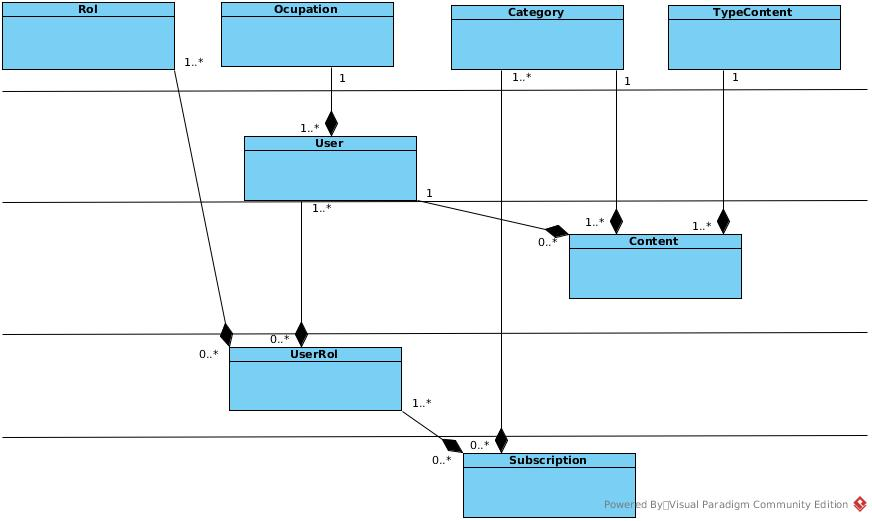
\includegraphics[scale=0.5]{subscriptionTest}
	}
	\captionof{figure}{Diagrama de clase representa la dependencia de suscripción}
	\source{fuente: (Elaboración propia)}
	\label{fig:Diagrama de clase representa la dependencia de suscripción}
\end{figure}

\end{itemize}

\subsection{Reporte de prueba}

\begin{itemize}

\item \textbf{Prueba unitaria de suscripción} únicamente, esta sección utiliza
el uso de reporte para especificar la ejecución.

Acorde con clase suscripción subsección \ref{serviceFeed}, se realiza la
prueba necesaria.

% report test 1
\begin{table}[!ht]\centering
\begin{tabular}{|c|c|}
\hline
\multicolumn{2}{|c|}{\textbf{Caso Prueba de Unidad}} \\ \hline
\multicolumn{1}{|l|}{Caso de prueba ID: 1} & \multicolumn{1}{l|}{Nombre de módulo: Categoría} \\ \hline
\multicolumn{1}{|l|}{Título prueba: executeOneLevelCategory} & \multicolumn{1}{l|}{Ejecución de prueba: 20-06-2016} \\ \hline
\multicolumn{1}{|l|}{Prioridad de prueba: Alto} & \multicolumn{1}{l|}{Fecha diseño de prueba: 11-02-2016} \\ \hline
\multicolumn{2}{|l|}{Pre-condición: BD vacía.} \\ \hline
\multicolumn{2}{|l|}{Dependencia: Categoría nivel zero.} \\ \hline
\textbf{Pasos de prueba} & \textbf{Datos de prueba} \\ \hline
\begin{tabular}[c]{@{}c@{}}Registrar categoría\\ de un nivel uno.\end{tabular} & \multicolumn{1}{l|}{\begin{tabular}[c]{@{}l@{}}nombre\_categoría='Quechua Psicosocial' \\ nombre\_url\_imagen\_categoría='psicosocial.jpg' \\ url\_imagen\_categoría='123\_psicosocial.jpg' \\ descripción\_categoría='descripción psicosocial' \\ descripción\_creditos='descripción creditos' \\ descripción\_objetivo='descripción objetivo' \\ categoría\_id\_categoría=6\end{tabular}} \\ \hline
\textbf{Resultado esperado} & \textbf{Resultado actual} \\ \hline
verdad & verdad \\ \hline
\textbf{Estado} & \textbf{Notas} \\ \hline
éxito & nombre categoría debe ser único. \\ \hline
\end{tabular}
\captionof{table}{Reporte prueba 1}
\source{fuente: (Elaboración propia)}
\label{Reporte prueba 1}
\end{table}

%report test 2
\begin{table}[H]\centering
\begin{tabular}{|c|c|}
\hline
\multicolumn{2}{|c|}{\textbf{Caso Prueba de Unidad}} \\ \hline
\multicolumn{1}{|l|}{Caso de prueba ID: 2} & \multicolumn{1}{l|}{Nombre de módulo: Ocupación} \\ \hline
\multicolumn{1}{|l|}{Título prueba: executeOcupation} & \multicolumn{1}{l|}{Ejecución de prueba: 20-06-2016} \\ \hline
\multicolumn{1}{|l|}{Prioridad de prueba: Alto} & \multicolumn{1}{l|}{Fecha diseño de prueba: 11-02-2016} \\ \hline
\multicolumn{1}{|l|}{Pre-condición: BD vacía.} & \multicolumn{1}{l|}{Dependencia: Ocupación nivel zero.} \\ \hline
\textbf{Pasos de prueba} & \textbf{Datos de prueba} \\ \hline
\begin{tabular}[c]{@{}c@{}}Registrar ocupación \\ de un nivel uno.\end{tabular} & \multicolumn{1}{l|}{\begin{tabular}[c]{@{}l@{}}nombre\_ocupación='Gerente de serivicos administrativos' \\ ocupación\_id\_ocupación=76\end{tabular}} \\ \hline
\textbf{Resultado esperado} & \textbf{Resultado actual} \\ \hline
verdad & verdad \\ \hline
\textbf{Estado} & \textbf{Notas} \\ \hline
éxito & nombre ocupación debe ser único. \\ \hline
\end{tabular}
\captionof{table}{Reporte prueba 2}
\source{fuente: (Elaboración propia)}
\label{Reporte prueba 2}
\end{table}

% report test 3
\begin{table}[!ht]\centering
\begin{tabular}{|c|c|}
\hline
\multicolumn{2}{|c|}{\textbf{Caso Prueba de Unidad}} \\ \hline
\multicolumn{1}{|l|}{Caso de prueba ID: 3} & \multicolumn{1}{l|}{Nombre de módulo: Rol} \\ \hline
\multicolumn{1}{|l|}{Título prueba: executeRol} & \multicolumn{1}{l|}{Ejecución de prueba: 20-06-2016} \\ \hline
\multicolumn{1}{|l|}{Prioridad de prueba: Alto} & \multicolumn{1}{l|}{Fecha diseño de prueba: 12-02-2016} \\ \hline
\multicolumn{1}{|l|}{Pre-condición: BD vacía.} & \multicolumn{1}{l|}{Dependencia:} \\ \hline
\textbf{Pasos de prueba} & \textbf{Datos de prueba} \\ \hline
Registrar nombre rol. & \multicolumn{1}{l|}{nombre\_rol='autorregulado'} \\ \hline
\textbf{Resultado esperado} & \textbf{Resultado actual} \\ \hline
verdad & verdad \\ \hline
\textbf{Estado} & \textbf{Notas} \\ \hline
éxito & nombre rol debe ser único. \\ \hline
\end{tabular}
\captionof{table}{Reporte prueba 3}
\source{fuente: (Elaboración propia)}
\label{Reporte prueba 3}
\end{table}

% report test 4
\begin{table}[H]\centering
\begin{tabular}{|c|c|}
\hline
\multicolumn{2}{|c|}{\textbf{Caso Prueba de Unidad}} \\ \hline
\multicolumn{1}{|l|}{Caso de prueba ID: 4} & \multicolumn{1}{l|}{Nombre de módulo: Usuario} \\ \hline
\multicolumn{1}{|l|}{Título prueba: executeUserOneLevelOcupation} & \multicolumn{1}{l|}{Ejecución de prueba: 20-06-2016} \\ \hline
\multicolumn{1}{|l|}{Prioridad de prueba: Alto} & \multicolumn{1}{l|}{Fecha diseño de prueba: 18-02-2016} \\ \hline
\multicolumn{1}{|l|}{Pre-condición: Usuario disponible.} & \multicolumn{1}{l|}{Dependencia: Ocupación.} \\ \hline
%\multicolumn{2}{|l|}{} \\ \hline
%\multicolumn{2}{|l|}{} \\ \hline
\textbf{Pasos de prueba} & \textbf{Datos de prueba} \\ \hline
Registrar datos de usuario. & \multicolumn{1}{l|}{\begin{tabular}[c]{@{}l@{}}correo='juan@gmail.com' \\ nombre\_usuario='omarhuanca' \\ contraseña='123' \\ estado\_usuario=1 \\ llaveActivación='1a2b3c' \\ ocupación\_id\_ocupación=84\end{tabular}} \\ \hline
\textbf{Resultado esperado} & \textbf{Resultado actual} \\ \hline
verdad & verdad \\ \hline
\textbf{Estado} & \textbf{Notas} \\ \hline
éxito & \begin{tabular}[c]{@{}c@{}}nombre\_usuario, correo \\ debe ser único.\end{tabular} \\ \hline
\end{tabular}
\captionof{table}{Reporte prueba 4}
\source{fuente: (Elaboración propia)}
\label{Reporte prueba 4}
\end{table}

% report test 5
\begin{table}[!ht]\centering
\begin{tabular}{|c|c|}
\hline
\multicolumn{2}{|c|}{\textbf{Caso Prueba de Unidad}} \\ \hline
\multicolumn{1}{|l|}{Caso de prueba ID: 5} & \multicolumn{1}{l|}{Nombre de módulo: Contenido} \\ \hline
\multicolumn{1}{|l|}{Título prueba: executeContentTypeAudio} & \multicolumn{1}{l|}{Ejecución de prueba: 20-06-2016} \\ \hline
\multicolumn{1}{|l|}{Prioridad de prueba: Medio} & \multicolumn{1}{l|}{Fecha diseño de prueba: 18-02-2016} \\ \hline
\multicolumn{2}{|l|}{Pre-condición: Usuario disponible, Contenido disponible.} \\ \hline
\multicolumn{2}{|l|}{Dependencia: Ocupación, Usuario, Categoría, TipoContenido.} \\ \hline
\textbf{Pasos de prueba} & \textbf{Datos de prueba} \\ \hline
Registrar datos de contenido. & \multicolumn{1}{l|}{\begin{tabular}[c]{@{}l@{}}título='Contenido 1' \\ fecha\_creación='2016-06-20 12:10:00' \\ fecha\_liberación='2016-06-21' \\ descripción='descripción' \\ nombre\_url\_imagen='imagen contenido 1' \\ url\_imagen='123\_imagen\_contenido\_1' \\ nombre\_url\_reproductor='reproductor contenido 1' \\ url\_reproductor='456\_reproductor\_1' \\ nombre\_url\_respuesta='documento respuesta 1' \\ url\_respuesta=789\_documento\_respuesta\_1' \\ nombre\_url\_glosario='documento glosario 1' \\ url\_glosario='1011\_documento\_glosario\_1' \\ créditos='créditos contenido 1' \\ contenido\_estado=1 \\ tipo\_contenido\_id\_tipo\_contenido=1 \\ categoría\_id\_categoría=28\end{tabular}} \\ \hline
\textbf{Resultado esperado} & \textbf{Resultado actual} \\ \hline
verdad & verdad \\ \hline
\textbf{Estado} & \textbf{Notas} \\ \hline
éxito & \begin{tabular}[c]{@{}c@{}}fecha liberación debe \\ ser mayora fecha de creación.\end{tabular} \\ \hline
\end{tabular}
\captionof{table}{Reporte prueba 5}
\source{fuente: (Elaboración propia)}
\label{Reporte prueba 5}
\end{table}

% report test 6
\begin{table}[H]\centering
\begin{tabular}{|c|c|}
\hline
\multicolumn{2}{|c|}{\textbf{Caso Prueba de Unidad}} \\ \hline
\multicolumn{1}{|l|}{Caso de prueba ID: 6} & \multicolumn{1}{l|}{Nombre de módulo: UsuarioRol} \\ \hline
\multicolumn{1}{|l|}{Título prueba: executeUserRol} & \multicolumn{1}{l|}{Ejecución de prueba: 20-06-2016} \\ \hline
\multicolumn{1}{|l|}{Prioridad de prueba: Medio} & \multicolumn{1}{l|}{Fecha diseño de prueba: 18-02-2016} \\ \hline
\multicolumn{2}{|l|}{Pre-condición: Usuario disponible.} \\ \hline
\multicolumn{2}{|l|}{Dependencia: Ocupación, Usuario, Rol.} \\ \hline
\textbf{Pasos de prueba} & \textbf{Datos de prueba} \\ \hline
Registrar datos de usuario\_rol. & \multicolumn{1}{l|}{\begin{tabular}[c]{@{}l@{}}usuario\_id\_usuario=35\\ rol\_id\_rol=7\end{tabular}} \\ \hline
\textbf{Resultado esperado} & \textbf{Resultado actual} \\ \hline
verdad & verdad \\ \hline
\textbf{Estado} & \textbf{Notas} \\ \hline
éxito &  \\ \hline
\end{tabular}
\captionof{table}{Reporte prueba 6}
\source{fuente: (Elaboración propia)}
\label{Reporte prueba 6}
\end{table}

% report test 7
\begin{table}[!ht]\centering
\begin{tabular}{|c|c|}
\hline
\multicolumn{2}{|c|}{\textbf{Caso Prueba de Unidad}} \\ \hline
\multicolumn{1}{|l|}{Caso de prueba ID: 7} & \multicolumn{1}{l|}{Nombre de módulo: Suscripción} \\ \hline
\multicolumn{1}{|l|}{Título prueba: executeSubscription} & \multicolumn{1}{l|}{Ejecución de prueba: 20-06-2016} \\ \hline
\multicolumn{1}{|l|}{Prioridad de prueba: Medio} & \multicolumn{1}{l|}{Fecha diseño de prueba: 18-02-2016} \\ \hline
\multicolumn{2}{|l|}{Pre-condición: Usuario disponible, Contenido disponible.} \\ \hline
\multicolumn{2}{|l|}{Dependencia: Ocupación, Usuario, Rol, UsuarioRol, Categoría.} \\ \hline
\textbf{Pasos de prueba} & \textbf{Datos de prueba} \\ \hline
Registrar datos de Suscripción. & \multicolumn{1}{l|}{\begin{tabular}[c]{@{}l@{}}categoría\_id\_categoría=7\\ id\_usuario\_rol=2\\ usuario\_id\_usuario=2\\ rol\_id\_rol=2\end{tabular}} \\ \hline
\textbf{Resultado esperado} & \textbf{Resultado actual} \\ \hline
verdad & verdad \\ \hline
\textbf{Estado} & \textbf{Notas} \\ \hline
éxito &  \\ \hline
\end{tabular}
\captionof{table}{Reporte prueba 7}
\source{fuente: (Elaboración propia)}
\label{Reporte prueba 7}
\end{table}

En la figura \ref{fig:Ejecución de prueba para registrar suscripción}, la prueba
ejecuta la verificación dependencias para crear una suscripción. 

\begin{figure}[!ht]
	\centering
	\fbox{
		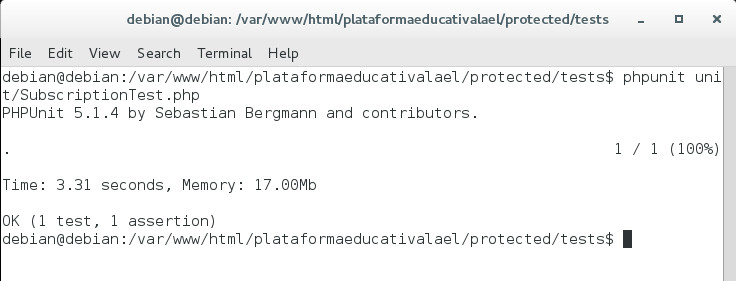
\includegraphics[scale=0.7]{runSubscriptionTest}
	}
	\captionof{figure}{Ejecución de prueba para registrar suscripción}
	\source{fuente: (Elaboración propia)}
	\label{fig:Ejecución de prueba para registrar suscripción}
\end{figure}


\item \textbf{Prueba integración de audio y vídeo}

% report test 8
\begin{table}[H]\centering
\begin{tabular}{|c|c|}
\hline
\multicolumn{2}{|c|}{\textbf{Caso Prueba de Integración}} \\ \hline
\multicolumn{1}{|l|}{Caso de prueba ID: 8} & \multicolumn{1}{l|}{Nombre de módulo: Contenido} \\ \hline
\multicolumn{1}{|l|}{Título prueba: playAudioLocalHost} & \multicolumn{1}{l|}{Ejecución de prueba: 23-05-2016} \\ \hline
\multicolumn{1}{|l|}{Prioridad de prueba: Bajo} & \multicolumn{1}{l|}{Fecha diseño de prueba: 13-03-2016} \\ \hline
\multicolumn{2}{|l|}{Pre-condición: Contenido disponible, phpunit disponible, selenium webdriver ejecutado.} \\ \hline
\multicolumn{2}{|l|}{Dependencia: Ocupación, Usuario, Rol, UsuarioRol, Categoría, TipoContenido.} \\ \hline
\textbf{Pasos de prueba} & \textbf{Datos de prueba} \\ \hline
Obtener URL de podcast de tipo audio. & \multicolumn{1}{l|}{\begin{tabular}[c]{@{}l@{}}http://localhost/plataformaeducativalael/content/\\ viewContent?id\_content=1\&user\_id\_user=27\&\\ type\_content\_id\_type\_content=1\&\\ category\_id\_category=2\end{tabular}} \\ \hline
\textbf{Resultado esperado} & \textbf{Resultado actual} \\ \hline
verdad & verdad \\ \hline
\textbf{Estado} & \textbf{Notas} \\ \hline
éxito &  \\ \hline
\end{tabular}
\captionof{table}{Reporte prueba 8}
\source{fuente: (Elaboración propia)}
\label{Reporte prueba 8}
\end{table}

% report test 9
\begin{table}[!ht]\centering
\begin{tabular}{|c|c|}
\hline
\multicolumn{2}{|c|}{\textbf{Caso Prueba de Integración}} \\ \hline
\multicolumn{1}{|l|}{Caso de prueba ID: 9} & \multicolumn{1}{l|}{Nombre de módulo: Contenido} \\ \hline
\multicolumn{1}{|l|}{Título prueba: playVideoLocalHost} & \multicolumn{1}{l|}{Ejecución de prueba: 23-05-2016} \\ \hline
\multicolumn{1}{|l|}{Prioridad de prueba: Bajo} & \multicolumn{1}{l|}{Fecha diseño de prueba: 15-03-2016} \\ \hline
\multicolumn{2}{|l|}{Pre-condición: Contenido disponible, phpunit disponible, selenium webdriver ejecutado.} \\ \hline
\multicolumn{2}{|l|}{Dependencia: Ocupación, Usuario, Rol, UsuarioRol, Categoría, TipoContenido.} \\ \hline
\textbf{Pasos de prueba} & \textbf{Datos de prueba} \\ \hline
Obtener URL de podcast de tipo vídeo. & \multicolumn{1}{l|}{\begin{tabular}[c]{@{}l@{}}http://localhost/plataformaeducativalael/content/\\ viewContent?id\_content=2\&user\_id\_user=27\&\\ type\_content\_id\_type\_content=2\&\\ category\_id\_category=3\end{tabular}} \\ \hline
\textbf{Resultado esperado} & \textbf{Resultado actual} \\ \hline
verdad & verdad \\ \hline
\textbf{Estado} & \textbf{Notas} \\ \hline
éxito &  \\ \hline
\end{tabular}
\captionof{table}{Reporte prueba 9}
\source{fuente: (Elaboración propia)}
\label{Reporte prueba 9}
\end{table}

En la figura \ref{fig:Ejecución de prueba para reproducir audio y vídeo}, la prueba
ejecuta la prueba de integración de audio y vídeo. 

%\begin{figure}[H]
\begin{figure}[H]
	\centering
	\fbox{
		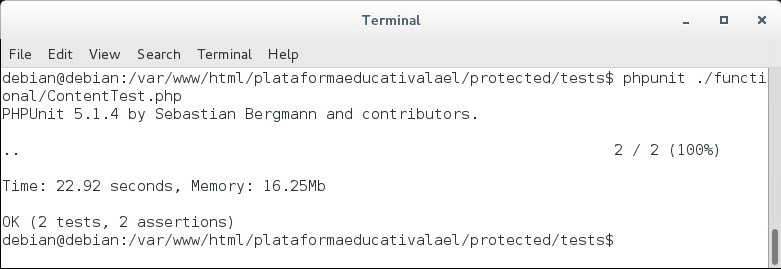
\includegraphics[scale=0.7]{runIntegrationTest}
	}
	\captionof{figure}{Ejecución de prueba para reproducir audio y vídeo}
	\source{fuente: (Elaboración propia)}
	\label{fig:Ejecución de prueba para reproducir audio y vídeo}
\end{figure}

\end{itemize}

\subsection{Implementar componente}

\begin{itemize}

\item \textbf{Prueba unitaria} se hace uso de phpunit.

\item \textbf{Prueba de integración} se hace uso de selenium server
standalone y un módulo webdriver-bindings \footnote{webdriver-bindings:
Permite ejecutar pruebas funcionales utilizando funciones WebDriver de
selenium server 2.0 se ejecuta como plug-in de navegador remoto,
por lo que es mucho más fiable que la prueba estándar de selenium se inyecta
a través de JavaScript. \cite{webdriverTest}}.

\end{itemize}

\begin{itemize}

\item \textbf{Prueba unitaria}

\begin{enumerate}

\item \textbf{Implementar en el servidor} la definición de la prueba
\textquotedouble{executeSubscription} comprueba la ejecución de una
suscripción, la descripción de la prueba se la aprecia en 
tabla \ref{Reporte prueba 7}.

\begin{lstlisting}[language=PHP, caption={Prueba de ejecución para suscripción.}]
class SubscriptionTest extends CDbTestCase {
    public function setUp() { // before each run test
        parent::setUp();
        ...
    }
    public function tearDown() { // after each run test
        parent::tearDown();
        ...
    }
    public function testCreateSubscription() {
        $subscription = new Subscription();     // create subscription
        $subscription->setAttributes(array(
        'category_id_category' => $this->categoryChild->id_category,
        'id_user_rol' => $this->userRol->id_user_rol,
        'user_id_user' => $this->userRol->user_id_user,
        'rol_id_rol' => $this->userRol->rol_id_rol
        ), false);
        $this->assertTrue($subscription->save(false));
    }
}
\end{lstlisting}

\item \textbf{Implementar en el servidor} la clase suscripción tiene una
función para control de excepción, se utilizó transacción \footnote{transacción:
Una secuencia de intercambio de información y el trabajo relacionado que se
trata como una unidad a efectos de satisfacer una solicitud como para
asegurar la integridad de la base de datos. \cite{transaction}} para manejo
de consistencia.

\begin{lstlisting}[language=PHP, caption={Función callback para control dependencia.}]
public function beforeSave() {
$res = false;
if ($this->isNewRecord) {
    $transaction = $this->dbConnection->beginTransaction(); // start transaction
    ...
    $category = Category::model()->findByAttributes(array('id_category' => 
        $this->category_id_category));
    if (isset($category)) {
        if (Yii::app()->params['idTypeContentAudio'] == 
                $this->type_content_id_type_content) {
            $user = User::model()->findByAttributes(array('id_user' => 
                $this->user_id_user, 'state_user' => Yii::app()->params[
                    'stateUserAvailable']));
            if (isset($user)) {
                $res = true;
            }
        }
    }
    if ($res) {
        $transaction->commit();
    } else {
        $transaction->rollback();
    }
    ...
} else {
    $res = true;
}
return $res;
}
\end{lstlisting}

\end{enumerate}

\item \textbf{Prueba de integración}

\begin{enumerate}

\item \textbf{Reproducir audio}

\begin{enumerate}

\item \textbf{Implementar en el servidor} la función de prueba
\textquotedouble{playAudioLocalHost} realiza la verificación de existencia
de un reproductor de tipo audio.

\begin{lstlisting}[language=PHP, caption={Prueba para reproducir reproductor de audio.}]
protected function setUp() {
    parent::setUp('localhost', 4444, 'firefox');
}
public function testPlayAudioLocalHost() {
    $this->get('http://localhost/plataformaeducativalael/content/'
    . 'viewContent/id_content/1/user_id_user/27/'
    . 'type_content_id_type_content/1/category_id_category/2');
    $this->click('audio-player');
    sleep(5);
    $elem = $this->findElementBy(LocatorStrategy::id,
        'audio-player');
    $this->assertNotNull($elem, 'Results not found!');
} 
\end{lstlisting}

\end{enumerate}

\item \textbf{Reproducir vídeo}

\begin{enumerate}

\item \textbf{Implementar en el servidor} la función de prueba
\textquotedouble{playVideoLocalHost} realiza la verificación de un reproductor
de tipo vídeo.

\begin{lstlisting}[language=PHP, caption={Prueba para reproducir reproductor de vídeo.}]
protected function setUp() {
    parent::setUp('localhost', 4444, 'firefox');
}
public function testPlayVideoLocalHost() {
    $this->get('http://localhost/plataformaeducativalael/content/'
    . 'viewContent?id_content=2&user_id_user=27&'
    . 'type_content_id_type_content=2&category_id_category=4');
    $this->click('audio-player');
    sleep(5);
    $elem = $this->findElementBy(LocatorStrategy::id,'audio-player');
    $this->assertNotNull($elem, 'Results not found!');
}
\end{lstlisting}

\end{enumerate}

\end{enumerate}

\end{itemize}

\subsection{Problema/Solución de componente}

\begin{itemize}

\item \textbf{Prueba unitaria}

\begin{itemize}

\item Instalar PHPUnit y dependencia desde composer.
\item Configurar archivos bootstrap y phpunit.xml sobre yii.
\item Editar archivos CWebTestCase para reconocimiento de sentencia phpunit.

\end{itemize}

\begin{enumerate}

\item \textbf{Uso dependencia phpunit} realizar la instalación de
dependencia para utilizar composer \footnote{composer: Es un gestor de
dependencias para PHP. Composer gestionará las dependencias que se requieren
en un proyecto por ejemplo. \cite{composer}}, a continuación se define la
ruta de instalación \textquotedouble{/project/protected/composer.json}

\begin{lstlisting}[caption={Dependencia de phpunit.}]
{
    "name": "kevin/protected",
    "authors": [
        {
            "name": "kevin",
            "email": "kevinflorenzdaus@gmail.com"
        }
    ],
    "require-dev": {
        "phpunit/phpunit": "3.7.*",
        "phpunit/phpunit-selenium": ">=1.2",
        "phpunit/dbunit": ">=1.2",
        "phpunit/phpunit-story": "*"
    }
}
\end{lstlisting}

\item \textbf{Configurar archivos bootstrap y phpunit}

Según \cite{testing} estos archivos son particulares, es como el guión de
entrada y es el punto de partida cuando se ejecuta una serie de pruebas.

\begin{lstlisting}[language=PHP, caption={Estructura de configuración de archivo bootstrap.}]
$vendors=dirname(__FILE__).'/../vendor/autoload.php';
$yiit=dirname(__FILE__).'/../../framework/yiit.php';
$config=dirname(__FILE__).'/../config/test.php'; //change the paths if necessary
require_once($vendors); // required file
require_once($yiit);
require_once(dirname(__FILE__).'/WebTestCase.php');
Yii::createWebApplication($config); // config app
\end{lstlisting}

En el segmento de código se representa la configuración de un archivo phpunit.xml
para uso de un navegador en específico.

\begin{lstlisting}[caption={Estructura de configuración archivo phpunit}]
<phpunit bootstrap="bootstrap.php"
	colors="false"
    convertErrorsToExceptions="true"
    convertNoticesToExceptions="true"
    convertWarningsToExceptions="true"
  	stopOnFailure="false">
<selenium>
	<browser name="Google Chrome" browser="*chrome" />
    <browser name="Firefox" browser="*firefox" />
</selenium>
</phpunit>
\end{lstlisting}

\item \textbf{Editar archivo CWebTestCase} el segmento de código muestra
el archivo CWebTestCase.php contempla tiene la configuración de inicio.

\begin{lstlisting}[language=PHP, caption={Cabecera de archivo CWebTestCase}, label={lst:fileCWebTestCase}]
Yii::import('system.test.CTestCase');
require_once('PHPUnit/Extensions/SeleniumTestCase.php');
\end{lstlisting}

A continuación el segmento de código muestra el archivo CWebTestCase.php
contiene una modificación. 

\begin{lstlisting}[language=PHP, caption={Modificación de instrucción.}, label={lst:replaceCWebTestCase}]
require_once('../../protected/vendor/phpunit/phpunit-selenium/
	PHPUnit/Extensions/SeleniumTestCase.php');
\end{lstlisting}

Como resultado, pruebas sobre Yii 1.X se debe realizar el cambio de sentencia
definido en segmento de código \ref{lst:replaceCWebTestCase}, por segmento de
código \ref{lst:fileCWebTestCase}.

\end{enumerate}

\item \textbf{Prueba integración}

\begin{itemize}

\item Instalación de navegador firefox.
\item Ejecutar sesión en selenium-server-standalone-Z.jar.
\item Inicio sesión en navegador chrome. 
 
\end{itemize}

\begin{enumerate}

\item \textbf{Instalación de navegador firefox} debian 8 utiliza un navegador
iceweasel reemplazar el por mozilla firefox.

\begin{lstlisting}[language=bash, caption={Instrucciones de instalación para mozilla firefox.}]
$ wget ftp://ftp.mozilla.org/pub/mozilla.org/..../firefox-Y.0.tar.bz2
cd /home/hugh/
$ tar -xjvf firefox-Y.0.tar.bz2
$ sudo rm -rf /opt/firefox*
$ sudo mv firefox /opt/firefoxY.0
$ sudo ln -sf /opt/firefoxY.0/firefox /usr/bin/firefox
\end{lstlisting}

La instalación de firefox tiene que ser de forma manual, un servidor web
como selenium-server-standalone-Z.jar utiliza la configuración de los
navegadores de uso general.

\item \textbf{Iniciar sesión selenium server standalone} el segmento de código
siguiente realiza el inicio del servidor web emulado.

\begin{lstlisting}[language=bash, caption={Ejecución de servidor server standalone.}]
$ java -jar  selenium-server-standalone-Z.jar
\end{lstlisting}

En la figura \ref{fig:Ejecución de selenium server standalone} selenium server
standalone empieza a funcionar.

%\begin{figure}[H]
\begin{figure}[!ht]
	\centering
	\fbox{
		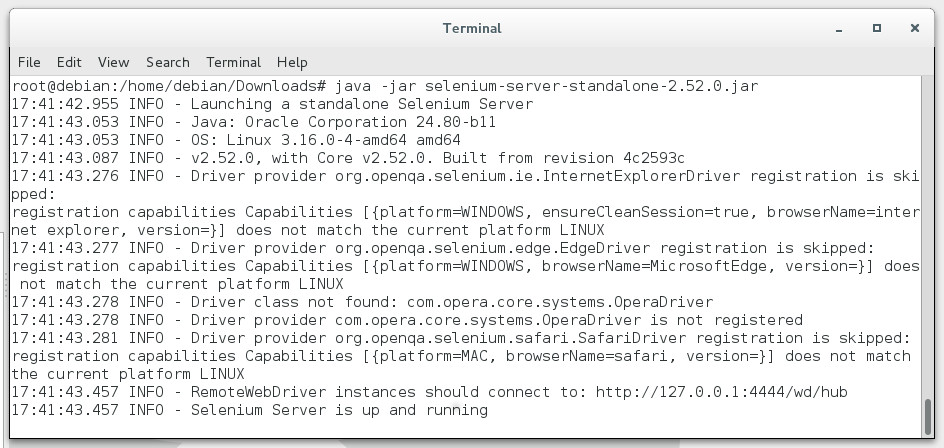
\includegraphics[scale=0.5]{executeSeleniumServer}
	}
	\captionof{figure}{Ejecución de selenium server standalone}
	\source{fuente: (Elaboración propia)}
	\label{fig:Ejecución de selenium server standalone}
\end{figure}

Realizar una  prueba de integración requiere ejecutar
\textquotedouble{dirección local} 
\footnote{dirección local: http://127.0.0.1:4444/wd/hub}, sobre un
navegador firefox, seleccionar la opción y crear una sesión de trabajo.

\item \textbf{Inicio sesión navegador en chrome} selenium server standalone
tiene una configuración por defecto con firefox, si se desea utilizar otro
navegador como alternativa. En el segmento de código se realiza la
configuración por medio de un programa de control de chrome para ejecución
de selenium server standalone.

A continuación se ejecuta los siguientes coman-dos de descarga.

\begin{lstlisting}[language=bash, caption={Instalación de programa de control para chrome.}]
$ unzip /path/chromedriver_linux_64.zip
$ su root
# chmod +x chromedriver
\end{lstlisting}

De manera que se tiene que ejecutar el siguiente comando en el siguiente
segmento de código \textquotedouble{sobre una sola línea}.

\begin{lstlisting}[language=bash, caption={Configuración chromedriver en selenium server.}]
$ java -jar selenium-server-standalone-Z.jar -Dwebdriver.chrome.driver=
"/path/chromedriver"
\end{lstlisting}

A continuación en la figura \ref{fig:Registro de sesión en navegador chrome},
se realiza la acción de inicio de sesión en chrome de ejecución de una prueba
de integración.

%\begin{figure}[H]
\begin{figure}[!ht]
	\centering
	\fbox{
		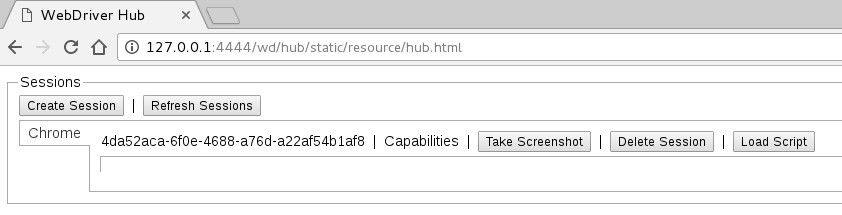
\includegraphics[scale=0.6]{registerSessionChrome}
	}
	\captionof{figure}{Registro de sesión en navegador chrome}
	\source{fuente: (Elaboración propia)}
	\label{fig:Registro de sesión en navegador chrome}
\end{figure}

En el segmento de código \ref{lst:configSetUpChrome}, en la línea tres se
tiene que reemplazar la instrucción \textquotedouble{firefox} por \textquotedouble{chrome}.

\begin{lstlisting}[language=PHP, caption={Configuración de ejecución de prueba para chrome.}, label={lst:configSetUpChrome}]
class ContentTest extends CWebDriverTestCase {
	protected function setUp() {
        parent::setUp('localhost', 4444, 'chrome');
    }
    ...
}
\end{lstlisting}

\end{enumerate}

\end{itemize}

\section{Duración proyecto}

Definir el tiempo de un sprint en 10 días hábiles para realizar la estimación
de esfuerzo del equipo desarrollo, en consideración se utilizo 21 sprints
para definir el siguiente orden de prioridad de las historias en tabla
\ref{tab:Product backlog - primera parte} y 
\ref{tab:Product backlog - segunda parte}.

% first part product backlog
\begin{table}[!ht]\centering
\begin{tabular}{|l|l|l|l|l|}
\hline
\multicolumn{1}{|c|}{\textbf{Historia}} & \multicolumn{1}{c|}{\textbf{Requerimiento}} & \multicolumn{1}{c|}{\textbf{Prioridad}} & \multicolumn{1}{c|}{\textbf{Programador}} & \multicolumn{1}{c|}{\textbf{Sprint}} \\ \hline
56 & Gestión de Ocupación. & Alto & Omar & 1 \\ \hline
06 & \begin{tabular}[c]{@{}l@{}}Registro manual deusuario aprendiz a la \\ plataforma.\end{tabular} & Alto & Omar & 1 \\ \hline
19 & \begin{tabular}[c]{@{}l@{}}Facilitar adaptación de plataforma al entorno\\ según al dispositivo.\end{tabular} & Alto & Rudy,Omar & 0 \\ \hline
05 & Registro por medio de red social. & Alto & Omar & 1 \\ \hline
10 & Identificación por medio de red social. & Alto & Omar & 1,2 \\ \hline
13 & Gestionar categoría. & Alto & Omar & 2,3,20 \\ \hline
16 & \begin{tabular}[c]{@{}l@{}}Generar menú de tipos de contenido por \\ categoría.\end{tabular} & Alto & Omar & 2,3 \\ \hline
57 & Gestión tipo contenido. & Alto & Omar & 2,4 \\ \hline
\end{tabular}
\captionof{table}{Product backlog - primera parte}
\source{fuente: (Elaboración propia)}
\label{tab:Product backlog - primera parte}
\end{table}

% second part product backlog
\begin{table}[!ht]\centering
\begin{tabular}{|l|l|l|l|l|}
\hline
\multicolumn{1}{|c|}{\textbf{Historia}} & \multicolumn{1}{c|}{\textbf{Requerimiento}} & \multicolumn{1}{c|}{\textbf{Prioridad}} & \multicolumn{1}{c|}{\textbf{Programador}} & \multicolumn{1}{c|}{\textbf{Sprint}} \\ \hline

21 & Gestión rol usuario tutor. & Alto & Rudy,Omar & 3,5 \\ \hline
22 & Gestión rol usuario coordinador. & Alto & Rudy,Omar & 3,4,5 \\ \hline
14 & \begin{tabular}[c]{@{}l@{}}Gestionar mi pregunta de selección múltiple\\ de contenido.\end{tabular} & Alto & Rudy,Omar & 3,5 \\ \hline

50 & Reiniciar contraseña de usuario. & Alto & Omar & 5 \\ \hline
31 & \begin{tabular}[c]{@{}l@{}}Gestionar mi preguntas de comprensión\\ en contenido.\end{tabular} & Alto & Rudy,Omar & 5 \\ \hline
32 & Gestionar mi pregunta de tipo juego en contenido. & Alto & Rudy,Omar & 6 \\ \hline
45 & \begin{tabular}[c]{@{}l@{}}Gestionar mi visualización gráfica de\\ contenido.\end{tabular} & Medio & Omar & 8,9 \\ \hline
30 & \begin{tabular}[c]{@{}l@{}}Gestionar mi pregunta de grabación en\\ contenido.\end{tabular} & Alto & Rudy,Omar & 5,9,10 \\ \hline
03 & \begin{tabular}[c]{@{}l@{}}Suscripción a una categoría.\end{tabular} & Medio & Omar & \begin{tabular}[c]{@{}l@{}}7,8\end{tabular} \\ \hline
65 & \begin{tabular}[c]{@{}l@{}}Suscripción a una categoría por red social.\end{tabular} & Medio & Omar & \begin{tabular}[c]{@{}l@{}}9,11\end{tabular} \\ \hline
11 & \begin{tabular}[c]{@{}l@{}}Animación transcripción en contenido de\\ tipo audio.\end{tabular} & Medio & Omar & 9 \\ \hline
59 & Liberación de contenidos & Medio & Omar & 9,10 \\ \hline
60 & \begin{tabular}[c]{@{}l@{}}Darse de baja suscripción podcast aprendiz\\ autorregulado.\end{tabular} & Bajo & Omar & 11 \\ \hline
44 & \begin{tabular}[c]{@{}l@{}}Animación transcripción en contenido de \\ tipo vídeo.\end{tabular} & Medio & Omar & 11 \\ \hline
33 & \begin{tabular}[c]{@{}l@{}}Gestionar pregunta de selección múltiple\\ en contenido.\end{tabular} & Alto & Rudy, Omar & 3,5 \\ \hline
34 & \begin{tabular}[c]{@{}l@{}}Gestionar pregunta de ordenamiento en \\ contenido.\end{tabular} & Alto & Rudy, Omar & 3,5 \\ \hline
35 & \begin{tabular}[c]{@{}l@{}}Gestionar pregunta de transcripción en\\ contenido.\end{tabular} & Alto & Rudy, Omar & 3,5 \\ \hline
36 & \begin{tabular}[c]{@{}l@{}}Gestionar pregunta de grabación en\\ contenido.\end{tabular} & Alto & Rudy, Omar & \begin{tabular}[c]{@{}l@{}}3,5,\\ 9,10\end{tabular} \\ \hline
37 & \begin{tabular}[c]{@{}l@{}}Gestionar pregunta de comprensión en\\ contenido.\end{tabular} & Alto & Rudy, Omar & 3,5 \\ \hline
61 & Registrar glosario audio podcast. & Medio & Omar & 13,14 \\ \hline
64 & Registrar subtitulado podcast. & Medio & Omar & 15,16 \\ \hline
66 & Gestión traducción transcripción en podcast. & Medio & Omar & 14,15,16 \\ \hline
62 & Implementar Prueba. & Bajo & Omar & \begin{tabular}[c]{@{}l@{}}16,17,18,\\19,21\end{tabular} \\ \hline
63 & Elaborar diccionario microformato. & Bajo & Omar & 20 \\ \hline
39 & \begin{tabular}[c]{@{}l@{}}Reproducción de audio de comprensión en\\ contenido.\end{tabular} & Alto & Rudy, Omar & 3 \\ \hline
12 & \begin{tabular}[c]{@{}l@{}}Representación de palabra en glosario de\\ contenido.\end{tabular} & Medio & Omar & 2 \\ \hline
42 & \begin{tabular}[c]{@{}l@{}}Animación de imagen de contenido vídeo\\ lado Front End.\end{tabular} & Medio & Omar & 2,11\\ \hline
48 & Gestionar visualización gráfica de contenido. & Medio & Omar & 2,9,15 \\ \hline
08 & \begin{tabular}[c]{@{}l@{}}Generar histograma de suscrito y visita\\ en mi contenido.\end{tabular} & Bajo & Omar &  \\ \hline
\end{tabular}
\captionof{table}{Product backlog - segunda parte}
\source{fuente: (Elaboración propia)}
\label{tab:Product backlog - segunda parte}
\end{table}